\documentclass{agujournal2019}
%DIF LATEXDIFF DIFFERENCE FILE
%DIF DEL papers/earths-future/submission_01.tex   Sat Jul  9 18:36:25 2022
%DIF ADD papers/earths-future/submission_02.tex   Wed Oct  5 10:56:13 2022

%% required packages
\usepackage{lineno}
\usepackage[inline]{trackchanges} %for better track changes. finalnew option will compile document with changes incorporated.

% Figures
\usepackage{graphicx}
\graphicspath{{../../plots/}{../../tikz/}{../../img/}}
\usepackage[section]{placeins} % require floats to appear in the section they are defined

% fonts and appearance
\usepackage{amsmath, amsfonts, physics, siunitx, nicefrac}

% better tables
\usepackage{booktabs}
\usepackage{array}
\newcommand{\PreserveBackslash}[1]{\let\temp=\\#1\let\\=\temp}
\newcolumntype{C}[1]{>{\PreserveBackslash\centering}p{#1}}
\newcolumntype{R}[1]{>{\PreserveBackslash\raggedleft}p{#1}}
\newcolumntype{L}[1]{>{\PreserveBackslash\raggedright}p{#1}}

% ACRONYMS
\usepackage[acronym, nopostdot, nonumberlist, shortcuts, numberedsection, nogroupskip,]{glossaries}
\newacronym{bfe}{BFE}{base flood elevation}
\newacronym{cmip}{CMIP}{the Coupled Model Intercomparison Project}
\newacronym{dmdu}{DMDU}{decision making under deep uncertainty}
\newacronym{fema}{FEMA}{the Federal Emergency Management Agency}
\newacronym{gev}{GEV}{generalized extreme value}
\newacronym{hazus}{HAZUS}{Hazard U.S.}
\newacronym{iid}{IID}{independent and identically distributed}
\newacronym{ipcc}{IPCC}{International Panel on Climate Change}
\newacronym{msl}{MSL}{mean relative sea level}
\newacronym{noaa}{NOAA}{the National Oceanic and Atmospheric Administration}
\newacronym{pdf}{PDF}{probability density function}
\newacronym{rcp}{RCP}{representative concentration pathway}
\newacronym{rdm}{RDM}{robust decision making}
\newacronym{slr}{SLR}{sea level rise}
\newacronym{ssp}{SSP}{shared socio-economic pathway}
\newacronym[]{usace}{USACE}{United States Army Corps of Engineers}
\newacronym[]{usgs}{USGS}{United States Geological Survey}
\newacronym[\glslongpluralkey={states of the world}]{sow}{SOW}{state of the world}

\usepackage{xspace}
\makeatletter
\DeclareRobustCommand\onedot{\futurelet\@let@token\@onedot}
\def\@onedot{\ifx\@let@token.\else.\null\fi\xspace}
\def\eg{\emph{e.g}\onedot} \def\Eg{\emph{E.g}\onedot}
\def\ie{\emph{i.e}\onedot} \def\Ie{\emph{I.e}\onedot}
\def\etc{\emph{etc}\onedot} \def\vs{\emph{vs}\onedot}
\newcommand{\usd}[1]{\SI{#1}[\$]{}}

%DIF 53-70d53
%DIF < % cite things in supplemental info file
%DIF < % see https://www.overleaf.com/learn/how-to/Cross_referencing_with_the_xr_package_in_Overleaf
%DIF < % it's a big strange for Overleaf!
%DIF < \usepackage{xr-hyper}
%DIF < \makeatletter
%DIF < \newcommand*{\addFileDependency}[1]{% argument=file name and extension
%DIF <   \typeout{(#1)}
%DIF <   \@addtofilelist{#1}
%DIF <   \IfFileExists{#1}{}{\typeout{No file #1.}}
%DIF < }
%DIF < \makeatother
%DIF < \newcommand*{\myexternaldocument}[1]{%
%DIF <     \externaldocument{#1}%
%DIF <     \addFileDependency{#1.tex}%
%DIF <     \addFileDependency{#1.aux}%
%DIF < }
%DIF < \myexternaldocument{supplemental}
%DIF < 
%DIF -------
% this goes last
\usepackage{cleveref}

\linenumbers
%%%%%%%
% As of 2018 we recommend use of the TrackChanges package to mark revisions.
% The trackchanges package adds five new LaTeX commands:
%
%  \note[editor]{The note}
%  \annote[editor]{Text to annotate}{The note}
%  \add[editor]{Text to add}
%  \remove[editor]{Text to remove}
%  \change[editor]{Text to remove}{Text to add}
%
% complete documentation is here: http://trackchanges.sourceforge.net/
%%%%%%%

%\draftfalse

%% Enter journal name below.
%% Choose from this list of Journals:
%
% JGR: Atmospheres
% JGR: Biogeosciences
% JGR: Earth Surface
% JGR: Oceans
% JGR: Planets
% JGR: Solid Earth
% JGR: Space Physics
% Global Biogeochemical Cycles
% Geophysical Research Letters
% Paleoceanography and Paleoclimatology
% Radio Science
% Reviews of Geophysics
% Tectonics
% Space Weather
% Water Resources Research
% Geochemistry, Geophysics, Geosystems
% Journal of Advances in Modeling Earth Systems (JAMES)
% Earth's Future
% Earth and Space Science
% Geohealth
%
% ie, \journalname{Water Resources Research}

\journalname{Earth's Future}
%DIF PREAMBLE EXTENSION ADDED BY LATEXDIFF
%DIF UNDERLINE PREAMBLE %DIF PREAMBLE
\RequirePackage[normalem]{ulem} %DIF PREAMBLE
\RequirePackage{color}\definecolor{RED}{rgb}{1,0,0}\definecolor{BLUE}{rgb}{0,0,1} %DIF PREAMBLE
\providecommand{\DIFadd}[1]{{\protect\color{blue}\uwave{#1}}} %DIF PREAMBLE
\providecommand{\DIFdel}[1]{{\protect\color{red}\sout{#1}}}                      %DIF PREAMBLE
%DIF SAFE PREAMBLE %DIF PREAMBLE
\providecommand{\DIFaddbegin}{} %DIF PREAMBLE
\providecommand{\DIFaddend}{} %DIF PREAMBLE
\providecommand{\DIFdelbegin}{} %DIF PREAMBLE
\providecommand{\DIFdelend}{} %DIF PREAMBLE
\providecommand{\DIFmodbegin}{} %DIF PREAMBLE
\providecommand{\DIFmodend}{} %DIF PREAMBLE
%DIF FLOATSAFE PREAMBLE %DIF PREAMBLE
\providecommand{\DIFaddFL}[1]{\DIFadd{#1}} %DIF PREAMBLE
\providecommand{\DIFdelFL}[1]{\DIFdel{#1}} %DIF PREAMBLE
\providecommand{\DIFaddbeginFL}{} %DIF PREAMBLE
\providecommand{\DIFaddendFL}{} %DIF PREAMBLE
\providecommand{\DIFdelbeginFL}{} %DIF PREAMBLE
\providecommand{\DIFdelendFL}{} %DIF PREAMBLE
\newcommand{\DIFscaledelfig}{0.5}
%DIF HIGHLIGHTGRAPHICS PREAMBLE %DIF PREAMBLE
\RequirePackage{settobox} %DIF PREAMBLE
\RequirePackage{letltxmacro} %DIF PREAMBLE
\newsavebox{\DIFdelgraphicsbox} %DIF PREAMBLE
\newlength{\DIFdelgraphicswidth} %DIF PREAMBLE
\newlength{\DIFdelgraphicsheight} %DIF PREAMBLE
% store original definition of \includegraphics %DIF PREAMBLE
\LetLtxMacro{\DIFOincludegraphics}{\includegraphics} %DIF PREAMBLE
\newcommand{\DIFaddincludegraphics}[2][]{{\color{blue}\fbox{\DIFOincludegraphics[#1]{#2}}}} %DIF PREAMBLE
\newcommand{\DIFdelincludegraphics}[2][]{% %DIF PREAMBLE
\sbox{\DIFdelgraphicsbox}{\DIFOincludegraphics[#1]{#2}}% %DIF PREAMBLE
\settoboxwidth{\DIFdelgraphicswidth}{\DIFdelgraphicsbox} %DIF PREAMBLE
\settoboxtotalheight{\DIFdelgraphicsheight}{\DIFdelgraphicsbox} %DIF PREAMBLE
\scalebox{\DIFscaledelfig}{% %DIF PREAMBLE
\parbox[b]{\DIFdelgraphicswidth}{\usebox{\DIFdelgraphicsbox}\\[-\baselineskip] \rule{\DIFdelgraphicswidth}{0em}}\llap{\resizebox{\DIFdelgraphicswidth}{\DIFdelgraphicsheight}{% %DIF PREAMBLE
\setlength{\unitlength}{\DIFdelgraphicswidth}% %DIF PREAMBLE
\begin{picture}(1,1)% %DIF PREAMBLE
\thicklines\linethickness{2pt} %DIF PREAMBLE
{\color[rgb]{1,0,0}\put(0,0){\framebox(1,1){}}}% %DIF PREAMBLE
{\color[rgb]{1,0,0}\put(0,0){\line( 1,1){1}}}% %DIF PREAMBLE
{\color[rgb]{1,0,0}\put(0,1){\line(1,-1){1}}}% %DIF PREAMBLE
\end{picture}% %DIF PREAMBLE
}\hspace*{3pt}}} %DIF PREAMBLE
} %DIF PREAMBLE
\LetLtxMacro{\DIFOaddbegin}{\DIFaddbegin} %DIF PREAMBLE
\LetLtxMacro{\DIFOaddend}{\DIFaddend} %DIF PREAMBLE
\LetLtxMacro{\DIFOdelbegin}{\DIFdelbegin} %DIF PREAMBLE
\LetLtxMacro{\DIFOdelend}{\DIFdelend} %DIF PREAMBLE
\DeclareRobustCommand{\DIFaddbegin}{\DIFOaddbegin \let\includegraphics\DIFaddincludegraphics} %DIF PREAMBLE
\DeclareRobustCommand{\DIFaddend}{\DIFOaddend \let\includegraphics\DIFOincludegraphics} %DIF PREAMBLE
\DeclareRobustCommand{\DIFdelbegin}{\DIFOdelbegin \let\includegraphics\DIFdelincludegraphics} %DIF PREAMBLE
\DeclareRobustCommand{\DIFdelend}{\DIFOaddend \let\includegraphics\DIFOincludegraphics} %DIF PREAMBLE
\LetLtxMacro{\DIFOaddbeginFL}{\DIFaddbeginFL} %DIF PREAMBLE
\LetLtxMacro{\DIFOaddendFL}{\DIFaddendFL} %DIF PREAMBLE
\LetLtxMacro{\DIFOdelbeginFL}{\DIFdelbeginFL} %DIF PREAMBLE
\LetLtxMacro{\DIFOdelendFL}{\DIFdelendFL} %DIF PREAMBLE
\DeclareRobustCommand{\DIFaddbeginFL}{\DIFOaddbeginFL \let\includegraphics\DIFaddincludegraphics} %DIF PREAMBLE
\DeclareRobustCommand{\DIFaddendFL}{\DIFOaddendFL \let\includegraphics\DIFOincludegraphics} %DIF PREAMBLE
\DeclareRobustCommand{\DIFdelbeginFL}{\DIFOdelbeginFL \let\includegraphics\DIFdelincludegraphics} %DIF PREAMBLE
\DeclareRobustCommand{\DIFdelendFL}{\DIFOaddendFL \let\includegraphics\DIFOincludegraphics} %DIF PREAMBLE
%DIF LISTINGS PREAMBLE %DIF PREAMBLE
\RequirePackage{listings} %DIF PREAMBLE
\RequirePackage{color} %DIF PREAMBLE
\lstdefinelanguage{DIFcode}{ %DIF PREAMBLE
%DIF DIFCODE_UNDERLINE %DIF PREAMBLE
  moredelim=[il][\color{red}\sout]{\%DIF\ <\ }, %DIF PREAMBLE
  moredelim=[il][\color{blue}\uwave]{\%DIF\ >\ } %DIF PREAMBLE
} %DIF PREAMBLE
\lstdefinestyle{DIFverbatimstyle}{ %DIF PREAMBLE
	language=DIFcode, %DIF PREAMBLE
	basicstyle=\ttfamily, %DIF PREAMBLE
	columns=fullflexible, %DIF PREAMBLE
	keepspaces=true %DIF PREAMBLE
} %DIF PREAMBLE
\lstnewenvironment{DIFverbatim}{\lstset{style=DIFverbatimstyle}}{} %DIF PREAMBLE
\lstnewenvironment{DIFverbatim*}{\lstset{style=DIFverbatimstyle,showspaces=true}}{} %DIF PREAMBLE
%DIF END PREAMBLE EXTENSION ADDED BY LATEXDIFF

\begin{document}

%% ------------------------------------------------------------------------ %%
%  Title
%
% (A title should be specific, informative, and brief. Use
% abbreviations only if they are defined in the abstract. Titles that
% start with general keywords then specific terms are optimized in
% searches)
%
%% ------------------------------------------------------------------------ %%

% Example: \title{This is a test title}

\title{A subjective Bayesian framework for synthesizing deep uncertainties in climate risk management}

%% ------------------------------------------------------------------------ %%
%
%  AUTHORS AND AFFILIATIONS
%
%% ------------------------------------------------------------------------ %%

\authors{James Doss-Gollin\affil{1}, Klaus Keller\affil{2}}
\affiliation{1}{Department of Civil and Environmental Engineering, Rice University}
\affiliation{2}{Thayer School of Engineering, Dartmouth College}

%% Corresponding Author:
% Corresponding author mailing address and e-mail address:

% (include name and email addresses of the corresponding author.  More
% than one corresponding author is allowed in this LaTeX file and for
% publication; but only one corresponding author is allowed in our
% editorial system.)

% Example: \correspondingauthor{First and Last Name}{email@address.edu}

\correspondingauthor{James Doss-Gollin}{jdossgollin@rice.edu}

\begin{keypoints}
  \item Decisions about how to manage climate risks are often made under deep uncertainty.
  \item We introduce a Bayesian framework to transparently synthesize and characterize deep uncertainties with the goal to support decision-making.
  \item We demonstrate the framework using a simple case study of \DIFdelbegin \DIFdel{house elevation for coastal flood risk management.
  }\DIFdelend \DIFaddbegin \DIFadd{how high to elevate a  house to manage coastal flood risks.
  }\item \DIFadd{Estimates of performance or robustness under deep uncertainty necessarily involve subjective judgments.
  }\DIFaddend \end{keypoints}


\begin{abstract}
  Projections of \DIFdelbegin \DIFdel{future }\DIFdelend \DIFaddbegin \DIFadd{nonstationary }\DIFaddend climate risks can vary considerably from one source to another, posing considerable communication and decision-analytical challenges.
  One such challenge is how to present trade-offs under deep uncertainty in a salient and interpretable manner.
  Some common approaches include analyzing a small subset of projections or \DIFdelbegin \DIFdel{invoking Laplace's principle of insufficient reason to justify a simple average}\DIFdelend \DIFaddbegin \DIFadd{treating all considered projections as equally likely}\DIFaddend .
  These approaches can underestimate risks, hide deep uncertainties, and \DIFdelbegin \DIFdel{provide little insight into }\DIFdelend \DIFaddbegin \DIFadd{are mostly silent on }\DIFaddend which assumptions drive decision-relevant outcomes.
  Here we introduce and demonstrate a transparent Bayesian framework for synthesizing deep uncertainties to inform climate risk management.
  The first step of this workflow is to generate an ensemble of simulations representing possible futures and analyze them through standard exploratory modeling techniques.
  Next, a small set of probability distributions representing subjective beliefs about the likelihood of possible futures is used to weight the scenarios.
  Finally, these weights are used to compute and characterize trade-offs, conduct robustness checks, and reveal implicit assumptions.
  We demonstrate the framework through a didactic case study analyzing how high to elevate a house to manage coastal flood risks.
\end{abstract}

\section*{Plain Language Summary}

\DIFdelbegin \DIFdel{The identification of }\DIFdelend \DIFaddbegin \DIFadd{Identifying }\DIFaddend sound strategies to manage risks driven by climatic changes is \DIFdelbegin \DIFdel{challenged by }\DIFdelend \DIFaddbegin \DIFadd{a complex task given the }\DIFaddend large uncertainties surrounding projections of  \DIFdelbegin \DIFdel{the }\DIFdelend coupled natural-human systems\DIFdelbegin \DIFdel{that influence projections of climate risk}\DIFdelend .
These uncertainties often arise from choices experts have to make, for example about how to formulate scientific models of future water levels.
Different experts can disagree about these choices, leading to different projections.
Analyzing decisions in such a situation of deep uncertainty poses nontrivial challenges.
For example, picking a single representative projection can \DIFdelbegin \DIFdel{lead to under-estimation of risk and }\DIFdelend \DIFaddbegin \DIFadd{under-estimate risk and result in }\DIFaddend poor decisions.
Similarly, communicating results separately for each projection can overwhelm decision-makers.
To make matters worse, typical approaches to this problem are mostly silent on what assumptions make a difference for the decisions at hand.
We develop and demonstrate a framework to address these challenges.
The framework provides a transparent approach to (i) combine a large number of deeply uncertain projections to a more \DIFdelbegin \DIFdel{understandable and smaller }\DIFdelend \DIFaddbegin \DIFadd{interpretable }\DIFaddend sample set and (ii) provide insights about which assumptions and modeling choices influence decisions.
We demonstrate the approach with a relatively simple example question of how high to elevate a house in the face of deeply uncertain projections of future water levels.

\DIFaddbegin \clearpage
\DIFaddend \section{Introduction}\label{sec:introduction}

\DIFdelbegin \DIFdel{Many critical infrastructure services around the world are aging \mbox{%DIFAUXCMD
    \cite<\eg,>{ho_dams:2017}}\hskip0pt%DIFAUXCMD
  .
  Moreover, }\DIFdelend \DIFaddbegin \DIFadd{Aging infrastructure and }\DIFaddend changes in regulations, finance, patterns of population and infrastructure use, and \DIFdelbegin \DIFdel{the climate system }\DIFdelend \DIFaddbegin \DIFadd{climate }\DIFaddend challenge the ability of critical infrastructures to meet design objectives \DIFdelbegin \DIFdel{\mbox{%DIFAUXCMD
    \cite{doss-gollin_txtreme:2021,doss-gollin_fatalism:2020,chester_reliable:2020}}\hskip0pt%DIFAUXCMD
  .
  The need to upgrade and expand infrastructure motivates the question: for which possible futures should infrastructure systems and components be designed?
  The answer to this question depends in part on values: intrinsic trade-offs between safety, performance , cost, and other objectives depend on context and stakeholder preferences \mbox{%DIFAUXCMD
    \cite{keller_management:2021} }\hskip0pt%DIFAUXCMD
  and are often regulated by statute or industry guidelines \mbox{%DIFAUXCMD
    \cite{bruneau_multihazard:2017}}\hskip0pt%DIFAUXCMD
  .
  For example, hospitals and critical infrastructure are generally designed to a higher standard of risk protection than ordinary buildings \mbox{%DIFAUXCMD
    \cite{asce_7-10:2013}}\hskip0pt%DIFAUXCMD
  .
  At the same time, performance depends upon future conditions, and so decisions about which scenario to design for are necessarily subject to implicit or explicit assumptions about the likelihood or possibility of different futures.
}%DIFDELCMD < 

%DIFDELCMD < %%%
\subsection{\DIFdel{Current practice}}
%DIFAUXCMD
\addtocounter{subsection}{-1}%DIFAUXCMD
%DIFDELCMD < 

%DIFDELCMD < %%%
\DIFdel{Current }\DIFdelend \DIFaddbegin \DIFadd{\mbox{%DIFAUXCMD
    \cite{doss-gollin_txtreme:2021,doss-gollin_fatalism:2020,chester_reliable:2020,asce_infrastructure_climate:2021,ho_dams:2017}}\hskip0pt%DIFAUXCMD
  .
  To achieve acceptable performance with reasonable planning efforts, current }\DIFaddend practice in engineering, infrastructure design, and \DIFdelbegin \DIFdel{local governance }\DIFdelend \DIFaddbegin \DIFadd{regulation }\DIFaddend relies heavily on standards that specify \DIFdelbegin \DIFdel{particular }\DIFdelend design events or conditions that buildings and infrastructure should safely withstand \DIFdelbegin \DIFdel{\mbox{%DIFAUXCMD
    \cite{asce_7-10:2013,bruneau_multihazard:2017}}\hskip0pt%DIFAUXCMD
  .
  These are often, though not always, informed by probabilistic analysis of relevant data.
}\DIFdelend \DIFaddbegin \DIFadd{\mbox{%DIFAUXCMD
    \cite{bruneau_multihazard:2017}}\hskip0pt%DIFAUXCMD
  .
}\DIFaddend For example, \gls{fema}, local governments, and engineering consultants produce local floodplain maps in many communities.
\DIFdelbegin \DIFdel{These trigger specific floodplain }\DIFdelend \DIFaddbegin \DIFadd{Buildings in the designated floodplain are subject to specific }\DIFaddend regulations, such as \DIFdelbegin \DIFdel{a requirement for homes in the 100-year floodplain with }\DIFdelend \DIFaddbegin \DIFadd{flood insurance requirements as an eligibility requirement for }\DIFaddend federally backed mortgages \DIFdelbegin \DIFdel{to be covered by flood insurance \mbox{%DIFAUXCMD
    \cite{kousky_voucher:2014} }\hskip0pt%DIFAUXCMD
  .
  Additionally, local building codes (based on guidance such as \mbox{%DIFAUXCMD
    \citeA{asce_24-05:2006} }\hskip0pt%DIFAUXCMD
  or \mbox{%DIFAUXCMD
    \citeA{FEMA_p-55:2011}}\hskip0pt%DIFAUXCMD
  ) may require new construction in flood zones to be elevated freeboard above a nominal \mbox{%DIFAUXCMD
    \gls{bfe}}\hskip0pt%DIFAUXCMD
  .
  Probabilistic analysis also informs the design of large-scale infrastructure.
  For example, some levees in the Netherlands are designed for a nominal annual failure probability of $\nicefrac{1}{4000}$ \mbox{%DIFAUXCMD
    \cite{eijgenraam_flooding:2014}}\hskip0pt%DIFAUXCMD
  , while a seawall proposed as part of a \$29 billion coastal protection project for  Galveston Bay was designed by setting the nominal annual probability of overtopping to 1\% \mbox{%DIFAUXCMD
    \cite[Appendix D.,~p.~2-59]{USACE_coastal:2021}}\hskip0pt%DIFAUXCMD
}\DIFdelend \DIFaddbegin \DIFadd{\mbox{%DIFAUXCMD
    \cite{kousky_voucher:2014} }\hskip0pt%DIFAUXCMD
  or minimum elevations for new construction \mbox{%DIFAUXCMD
    \cite{asce_24-05:2006,FEMA_p-55:2011}}\hskip0pt%DIFAUXCMD
  .
  Although this paper focuses on flooding, similar approaches inform mitigation strategies for a wide range of other hazards \mbox{%DIFAUXCMD
    \cite{asce_7-10:2013}}\hskip0pt%DIFAUXCMD
}\DIFaddend .

\DIFdelbegin \DIFdel{There are many advantagesto standards-based design.
  In particular, these heuristics are scalable and explainable, they reduce the complexity of design analysis, and they are fair in at least a procedural sense}\DIFdelend \DIFaddbegin \DIFadd{Standards-based risk management frameworks have many advantages, including scalability, explainability, and simplicity}\DIFaddend .
However, \DIFdelbegin \DIFdel{reliance on these heuristics also faces limitations.
  In particular, this sort of one-size-fits-all guidance may not be an efficient or desirable way to balance trade-offs between metrics of stakeholder values such as sense of place, distributive justice, economic efficiency, and safety \mbox{%DIFAUXCMD
    \cite{keller_management:2021}}\hskip0pt%DIFAUXCMD
  .
  This has motivated economically informed approaches, like risk-based }\DIFdelend \DIFaddbegin \DIFadd{the choice of standard is a complex design and policy choice.
  Risk-based }\DIFaddend design and cost benefit analysis \cite{eijgenraam_flooding:2014,vandantzig_dike:1956,xian_elevation:2017} \DIFdelbegin \DIFdel{, that place ``a strong emphasis upon a }\DIFdelend \DIFaddbegin \DIFadd{offer a quantitative framework for comparing possible standards by emphasizing ``a }\DIFaddend proportionate response to risk, so that the amount invested in risk reduction is in proportion to the magnitude of the risk and the cost-effectiveness with which that risk may be reduced'' \cite{merz_fluvial:2010}.
\DIFdelbegin \DIFdel{These quantitative cost-benefit analyses also rely on probabilistic descriptions of relevant hazard, and can be particularly sensitive to representation of tail probabilities \mbox{%DIFAUXCMD
    \cite{merz_heavytails:2022,wong_floodrisk:2018,garner_slrise:2018}}\hskip0pt%DIFAUXCMD
}\DIFdelend \DIFaddbegin \DIFadd{This provides a formal basis for choices such as protecting hospitals and critical infrastructure to a higher degree than ordinary buildings \mbox{%DIFAUXCMD
    \cite{asce_7-10:2013}}\hskip0pt%DIFAUXCMD
  .
  However, these methods are silent on how standards should balance trade-offs, not only between cost and performance but also between other stakeholder values such as sense of place, distributive justice, and safety \mbox{%DIFAUXCMD
    \cite{keller_management:2021,helgeson_manifesto:2022,quinn_rivalframings:2017,bessette_vimm:2017,vezer_epistemic:2018}}\hskip0pt%DIFAUXCMD
}\DIFaddend .

\DIFdelbegin \DIFdel{The approaches currently used to estimate the \mbox{%DIFAUXCMD
    \glspl{pdf} }\hskip0pt%DIFAUXCMD
  of climate hazards used in standard-setting and decision-making emphasize }\DIFdelend \DIFaddbegin \DIFadd{Moreover, estimates of performance trade-offs require implicit or explicit assumptions about the likelihood of different possible futures.
  Current practice emphasizes }\DIFaddend nominally objective methods that can be applied consistently across locations.
For example, \DIFaddbegin \DIFadd{the }\DIFaddend \gls{usgs} Bulletin 17C specifies procedures for estimating flood frequency \cite{bulletin17c:2019}\DIFdelbegin \DIFdel{and }\DIFdelend \DIFaddbegin \DIFadd{.
  Similarly, }\DIFaddend \gls{noaa} Atlas 14 provides estimates of the intensity, duration, and frequency of extreme rainfall \DIFdelbegin \DIFdel{\mbox{%DIFAUXCMD
    \cite{atlas14_texas:2018}}\hskip0pt%DIFAUXCMD
  .
  Among several statistical assumptions }\DIFdelend \DIFaddbegin \DIFadd{\mbox{%DIFAUXCMD
    \cite{atlas14_texas:2018,noaa_nonstationary:2022}}\hskip0pt%DIFAUXCMD
  .
  One statistical assumption }\DIFaddend these analyses make \DIFdelbegin \DIFdel{that have been recently called into question is stationarity \mbox{%DIFAUXCMD
    \cite<the assumption that past and future hazard come from the same \gls{pdf}; see>[for a review]{merz_review:2014}}\hskip0pt%DIFAUXCMD
  .
  For example, clear trends in extreme rainfall are apparent across much of southeastern Texas \mbox{%DIFAUXCMD
    \cite{fagnant_spatiotemporal:2020,nielsen-gammon_txrainfall:2020}}\hskip0pt%DIFAUXCMD
  , and trends in many other hazards for other locations are consistent with observations \mbox{%DIFAUXCMD
    \cite<see>[for a comprehensive summary]{ipcc_impacts:2022}}\hskip0pt%DIFAUXCMD
}\DIFdelend \DIFaddbegin \DIFadd{is stationarity (the assumption that past and future hazard come from the same \mbox{%DIFAUXCMD
    \gls{pdf}}\hskip0pt%DIFAUXCMD
  ), but global climate change and local environmental changes have cast scrutiny on this assumption \mbox{%DIFAUXCMD
    \cite{merz_review:2014,milly_stationarity:2008,doss-gollin_robustadaptation:2019}}\hskip0pt%DIFAUXCMD
}\DIFaddend .
While some methods have been proposed for incorporating \DIFdelbegin \DIFdel{trends into these }\DIFdelend \DIFaddbegin \DIFadd{nonstationarity into risk }\DIFaddend analyses \cite<see>[for a review]{Salas:2018ge}, these assume specific forms of \DIFdelbegin \DIFdel{nonstationarity }\DIFdelend \DIFaddbegin \DIFadd{a trend }\DIFaddend which may not \DIFdelbegin \DIFdel{fully }\DIFdelend \DIFaddbegin \DIFadd{adequately }\DIFaddend represent physical processes or \DIFdelbegin \DIFdel{true levels of uncertainty \mbox{%DIFAUXCMD
    \cite{doss-gollin_robustadaptation:2019,Montanari:2014hl,Serinaldi:2015bq}}\hskip0pt%DIFAUXCMD
  .
  Ultimately, the difficulty of incorporating nonstationarity into existing frameworks has led to continued reliance on stationarity despite recognition of the associated limitations as discussed in p.~2 of \mbox{%DIFAUXCMD
    \citeA{bulletin17c:2019} }\hskip0pt%DIFAUXCMD
  and p.~A.4-42 of \mbox{%DIFAUXCMD
    \citeA{atlas14_texas:2018}}\hskip0pt%DIFAUXCMD
  .
}%DIFDELCMD < 

%DIFDELCMD < %%%
\subsection{\DIFdel{Emerging paradigms}}
%DIFAUXCMD
\addtocounter{subsection}{-1}%DIFAUXCMD
%DIFDELCMD < 

%DIFDELCMD < %%%
\DIFdel{Projecting nonstationary hazard is difficult because many future hazards depend on human decisions (}%DIFDELCMD < \eg%%%
\DIFdel{, future greenhouse gas emissions) or on physical processes that are poorly constrained by existing data \mbox{%DIFAUXCMD
    \cite<\eg, collapse of the West Antarctic ice sheet;>[]{deconto_antarctica:2016}}\hskip0pt%DIFAUXCMD
  .
  In other words, they are deeply uncertain \mbox{%DIFAUXCMD
    \cite{keller_management:2021,walker_deep:2013,lempert_complex:2002,haasnoot_sealevelrise:2021}}\hskip0pt%DIFAUXCMD
  .
  These deeply uncertain nonstationary hazards challenge not only the existing stationary estimates but, more fundamentally, the premise that objective estimates }\DIFdelend \DIFaddbegin \DIFadd{sample only a subset of uncertainties \mbox{%DIFAUXCMD
    \cite{doss-gollin_robustadaptation:2019,montanari_immortal:2014,serinaldi_undead:2015}}\hskip0pt%DIFAUXCMD
  .
  At least in part because of the challenges associated with developing objective methods to select from diverging projections }\DIFaddend of future hazard\DIFdelbegin \DIFdel{exist and can be estimated empirically.
}\DIFdelend \DIFaddbegin \DIFadd{, official guidance continues to rely on the stationarity assumption \mbox{%DIFAUXCMD
    \cite{bulletin17c:2019,atlas14_texas:2018}}\hskip0pt%DIFAUXCMD
  .
}\DIFaddend

\DIFdelbegin \DIFdel{Recognizing the challenges of \mbox{%DIFAUXCMD
    \gls{dmdu}}\hskip0pt%DIFAUXCMD
  , many frameworks for identifying robust decisions have been proposed.
  Most emphasize the use of models in an exploratory (``what-if'') framework to learn about interactions between decisions and system dynamics \mbox{%DIFAUXCMD
    \cite{bankes:1993}}\hskip0pt%DIFAUXCMD
  .
  For example, robust decision making \mbox{%DIFAUXCMD
    \cite{lempert_shaping:2003} }\hskip0pt%DIFAUXCMD
  evaluates models over large ensembles of possible futures to assess the performance of different policies under each, then applies statistical analysis to identify the conditions under which particular policies perform well or poorly.
  When the decision space is complex, many analyses use policy search (often using multi-objective optimization tools) to identify promising actions \mbox{%DIFAUXCMD
    \cite{kasprzyk:2013,kasprzyk_denovo:2012,hadka_mordm:2015}}\hskip0pt%DIFAUXCMD
  .
  In addition, many studies formally quantify robustness to deep uncertainties \mbox{%DIFAUXCMD
    \cite{herman:2015,mcphail_robustness:2019} }\hskip0pt%DIFAUXCMD
  and use this as a criterion for policy comparison.
}%DIFDELCMD < 

%DIFDELCMD < %%%
\DIFdel{Although these \mbox{%DIFAUXCMD
    \gls{dmdu} }\hskip0pt%DIFAUXCMD
  methods have proven valuable in a wide range of settings, they still require necessarily subjective assessments about the likelihood of future conditions.
  Even exploratory models require the analyst to choose which uncertainties are considered and how they are sampled.
  When analyses use metrics that integrate performance over many possible futures, whether to compute sensitivities, estimate expectations, or compute robustness metrics, they necessarily make assumptions about the likelihood of different futures.
  For example, uniform priors are often justified by deferring to Laplace's principle of insufficient reason \mbox{%DIFAUXCMD
    \cite<see>[p.~135]{stigler_uncertainty:1986}}\hskip0pt%DIFAUXCMD
  , but even this choice makes strong assumptions that are sensitive to factors such as parameterization \mbox{%DIFAUXCMD
    \cite[p.54]{gelman_bda3:2014}}\hskip0pt%DIFAUXCMD
  .
  While one interpretation of deep uncertainty is that that specifying a joint \mbox{%DIFAUXCMD
    \gls{pdf} }\hskip0pt%DIFAUXCMD
  over inputs is inappropriate, assumptions about the ranges and independence of parameters to sample are just as subjective as the choice of probability distribution \mbox{%DIFAUXCMD
    \cite{schneider_scenarios:2002,quinn_exploratory:2020} }\hskip0pt%DIFAUXCMD
  and can often be interpreted  as a specific choice of probability distribution (we revisit this point in \mbox{%DIFAUXCMD
    \cref{sec:analysis-condition}}\hskip0pt%DIFAUXCMD
  ).
  This motivates the development of decision analytic frameworks that draw from the strengths of \mbox{%DIFAUXCMD
    \gls{dmdu} }\hskip0pt%DIFAUXCMD
  methods such as exploratory modeling, vulnerability assessment, robustness checks, and iterative stakeholder critique, but that embrace the reality that assumptions about the future are inescapable.
}%DIFDELCMD < 

%DIFDELCMD < %%%
\subsection{\DIFdel{Research gaps and objectives}}
%DIFAUXCMD
\addtocounter{subsection}{-1}%DIFAUXCMD
%DIFDELCMD < 

%DIFDELCMD < %%%
\DIFdel{We are motivated by parallels between decision making under deep uncertainty and the statistical problem of model selection.
  \mbox{%DIFAUXCMD
    \citeA{oreskes_verification:1994} }\hskip0pt%DIFAUXCMD
  argues that because natural }\DIFdelend \DIFaddbegin \DIFadd{The limitations of objectivist approaches to projecting risk extend beyond estimating nonstationary climate hazards.
  Human-natural }\DIFaddend systems are never closed and model results are never unique, \DIFaddbegin \DIFadd{and thus }\DIFaddend validation and verification of models representing these systems is necessarily qualitative and subjective \DIFdelbegin \DIFdel{.
  In the literature on decision making under deep uncertainty, this has led to recognition of the need to develop strategies }\DIFdelend \DIFaddbegin \DIFadd{\mbox{%DIFAUXCMD
    \cite{oreskes_verification:1994}}\hskip0pt%DIFAUXCMD
  .
  In other words, no model exists that could represent the full truth, and the future is thus deeply uncertain \mbox{%DIFAUXCMD
    \cite{keller_management:2021,walker_deep:2013,lempert_complex:2002,haasnoot_sealevelrise:2021}}\hskip0pt%DIFAUXCMD
  .
  Consequently, a growing literature on \mbox{%DIFAUXCMD
    \gls{dmdu} }\hskip0pt%DIFAUXCMD
  emphasizes the value of identifying decisions }\DIFaddend that are robust\DIFaddbegin \DIFadd{, in some sense, to deep uncertainties \mbox{%DIFAUXCMD
    \cite{moody_robustness:2013,herman:2015,mcphail_robustness:2019,borgomeo_robustness:2018}}\hskip0pt%DIFAUXCMD
  .
  Within this literature has emerged a debate regarding the value and use of probabilistic information  \mbox{%DIFAUXCMD
    \cite<see>[and references therein]{taner_probabilistic:2019}}\hskip0pt%DIFAUXCMD
  .
  On the one hand, scholars have pointed out that predictions are inherently unreliable, and representing deep uncertainties through probability distributions frequently over-estimates predictive skill \mbox{%DIFAUXCMD
    \cite{groves_scenarios:2007,lempert_robust:2000}}\hskip0pt%DIFAUXCMD
  .
  On the other, assessments of which decisions are robust depend on subjective choices about how to define robustness and how to sample uncertainties \mbox{%DIFAUXCMD
    \cite{mcphail_robustness:2019,quinn_exploratory:2020,schneider_scenarios:2002,schneider_dangerous:2001,reis_distribution:2020}}\hskip0pt%DIFAUXCMD
  .
}

\DIFadd{In this paper we offer a conceptual step towards bridging this divide by presenting a framework that is designed to combine the strengths of both approaches.
  In the first step, exploratory or bottom-up modeling is used }\DIFaddend to \DIFdelbegin \DIFdel{model imperfections.
  There are parallels to this challenge in the Bayesian literature on model selection, particularly in the ``$\mathcal{M}$-open'' case in which there is no ``true'' model to identify and all models are imperfect representations of reality.
  This is a theoretical contrast to the ``$\mathcal{M}$-closed'' case in which the data are assumed to come from a ``true'' model which is a member of the finite set of candidate models available to the analyst \mbox{%DIFAUXCMD
    \cite{bernardo_bayesian:1994}}\hskip0pt%DIFAUXCMD
  .
  Commonly used classical methods for model selection implicitly assume $\mathcal{M}$-closed case and are defined by their ability to asymptotically identify the true model from a set of candidate models.
  By contrast, model selection in the $\mathcal{M}$-open case emphasizes a subjective view of the modeling process, for which probability offers a }\DIFdelend \DIFaddbegin \DIFadd{build insight and identify potential system vulnerabilities \mbox{%DIFAUXCMD
    \cite{moallemi_exploratory:2020,bankes:1993,brown_decisionscaling:2012}}\hskip0pt%DIFAUXCMD
  .
  In the second step, we synthesize the results of exploratory modeling to formally estimate performance metrics and trade-offs using probabilistic models for uncertainty.
  Drawing from the literature on building predictive models when all models are wrong \mbox{%DIFAUXCMD
    \cite{box_sciencestatistics:1976,gelman_philosophy:2013,Piironen:2017eh}}\hskip0pt%DIFAUXCMD
  , we interpret these probability distributions not as statements of fact, but rather as a }\DIFaddend self-consistent \DIFdelbegin \DIFdel{language with which to reason about the unknown rather than a statement of objective truth (see \mbox{%DIFAUXCMD
    \citeA{gelman_philosophy:2013}}\hskip0pt%DIFAUXCMD
  , \mbox{%DIFAUXCMD
    \citeA{ramsey_probability:2016}}\hskip0pt%DIFAUXCMD
  , or \mbox{%DIFAUXCMD
    \citeA{jaynes_probability:2003} }\hskip0pt%DIFAUXCMD
  for a discussion of Bayesian philosophy and \mbox{%DIFAUXCMD
    \citeA{Piironen:2017eh} }\hskip0pt%DIFAUXCMD
  for a technical discussion of methods for model selection).
  From a practical perspective, model selection in the $\mathcal{M}$-open case emphasizes building models iteratively, simulating the consequences of these models , and subsequently using these simulations to critique and improve them until an acceptable model (in the analyst's subjective judgement) is reached \mbox{%DIFAUXCMD
    \cite{gelman_workflow:2020}}\hskip0pt%DIFAUXCMD
  .
  Thus, where classical statistics, particularly as applied to environmental systems, has often emphasized objectivity, we draw from this Bayesian literature that emphasizes a focus on building transparency in the presentation, analysis , and critique of models and results}\DIFdelend \DIFaddbegin \DIFadd{framework for reasoning about how different assumptions lead to different inferences.
  An advantage of our approach is that it facilitates computationally efficient analysis of how alternative probabilistic models would affect estimated performance metrics and trade-offs}\DIFaddend .

\DIFdelbegin \DIFdel{In this paper we offer a first conceptual step towards bridging the fields of \mbox{%DIFAUXCMD
    \gls{dmdu} }\hskip0pt%DIFAUXCMD
  and Bayesian model building.
  We consider }\DIFdelend \DIFaddbegin \DIFadd{We illustrate our approach through }\DIFaddend a didactic case study of whether to elevate a hypothetical house, and if so how high\DIFdelbegin \DIFdel{, as a specific example of a decision problem subject to both shallow (storm surge) and deep (\mbox{%DIFAUXCMD
    \gls{slr}}\hskip0pt%DIFAUXCMD
  ) uncertainties}\DIFdelend .
Prior studies have found that floodproofing and building-scale vulnerability reduction measures, including house elevation, can effectively reduce local flood damages in many contexts \cite{demoel_reducing:2014,deruig_building:2020,kreibich_building:2005,slotter_floodproofing:2020,rozer_coping:2016,mobley_mitigation:2020,aerts_cost:2018}, and both local building codes \cite{asce_7-10:2013,bruneau_multihazard:2017,asce_24-05:2006} and federal policy \cite{FEMA_p-55:2011} require elevation in some cases.
Guidance for homeowners, notably from \gls{fema}, recommends elevating to the \gls{bfe} (typically the \SI{100}{year} flood) plus a freeboard \cite{fema_retrofitting:2014,asce_24-14:2015,fema_retrofitting:2014} but recent research has demonstrated that neglecting uncertainty in the cost-benefit analysis can lead to poor decisions \cite{zarekarizi_suboptimal:2020}.
Focusing on deep uncertainty in \gls{slr} over the 70 year design life of a hypothetical house, we seek to answer the research question ``\emph{how can \DIFdelbegin \DIFdel{deep uncertainties be transparently synthesized for }\DIFdelend decision analysis \DIFaddbegin \DIFadd{transparently synthesize deep uncertainties}\DIFaddend ?}''
\DIFaddbegin \DIFadd{To shed light on this question in a single paper, we necessarily are silent on key issues that would be relevant to real-world decision-makers including alternative decision levers, the potential for adaptive decision rules, and rival problem framings.
}\DIFaddend

We proceed as follows.
In \cref{sec:analysis} we present three formal decision analytic frameworks for analyzing an ensemble of \gls{slr} simulations, building through existing approaches for exploratory modeling \DIFdelbegin \DIFdel{(\mbox{%DIFAUXCMD
    \cref{sec:analysis-explore}}\hskip0pt%DIFAUXCMD
  ) and scenario analysis (\mbox{%DIFAUXCMD
    \cref{sec:analysis-condition}}\hskip0pt%DIFAUXCMD
  ) towards a formal Bayesian method }\DIFdelend \DIFaddbegin \DIFadd{scenario analysis to identify a need for synthesizing across scenarios.
  We present a formal framework }\DIFaddend for transparently synthesizing deep \DIFdelbegin \DIFdel{uncertainty through subjective prior beliefs (\mbox{%DIFAUXCMD
    \cref{sec:analysis-synthesize}}\hskip0pt%DIFAUXCMD
  )}\DIFdelend \DIFaddbegin \DIFadd{uncertainties in \mbox{%DIFAUXCMD
    \cref{sec:reweighting}}\hskip0pt%DIFAUXCMD
}\DIFaddend .
In \cref{sec:case-study} we describe the \DIFdelbegin \DIFdel{case study in detail.
  Nextin \mbox{%DIFAUXCMD
    \cref{sec:results} }\hskip0pt%DIFAUXCMD
}\DIFdelend \DIFaddbegin \DIFadd{didactic case study.
  Next, in \mbox{%DIFAUXCMD
    \cref{sec:results}}\hskip0pt%DIFAUXCMD
  , }\DIFaddend we present results for each of the three decision lenses and discuss the advantages and limitations of each theoretical approach.
In \cref{sec:caveats} we discuss limitations of the study and future research needs.
Finally in \cref{sec:conclusions} we discuss key findings and implications for policy and practice.

\section{\DIFdelbegin \DIFdel{Decision analytic }\DIFdelend \DIFaddbegin \DIFadd{Conceptual }\DIFaddend framework}\label{sec:analysis}

In this section we \DIFdelbegin \DIFdel{outline our framework }\DIFdelend \DIFaddbegin \DIFadd{introduce a conceptual framework and notation }\DIFaddend for decision analysis under deep uncertainty\DIFdelbegin \DIFdel{, maintaining a high level of generality.
  In the next we discuss application to the house elevation case study.
}\DIFdelend \DIFaddbegin \DIFadd{.
  We then apply this framework to understand exploratory modeling (\mbox{%DIFAUXCMD
    \cref{sec:analysis-explore}}\hskip0pt%DIFAUXCMD
  ) and scenario-conditional probabilistic analysis (\mbox{%DIFAUXCMD
    \cref{sec:analysis-condition}}\hskip0pt%DIFAUXCMD
  ).
  In \mbox{%DIFAUXCMD
    \cref{sec:analysis-synthesize} }\hskip0pt%DIFAUXCMD
  we discuss why synthesizing across multiple scenarios is necessary.
  In \mbox{%DIFAUXCMD
    \cref{sec:reweighting} }\hskip0pt%DIFAUXCMD
  we provide a formal method for synthesizing across scenarios.
}\DIFaddend

\DIFaddbegin \DIFadd{It is common in climate risk management to work with an ensemble of trajectories of climate, economic, and other key variables, which we refer to as \mbox{%DIFAUXCMD
    \glspl{sow}}\hskip0pt%DIFAUXCMD
  .
  Often these \mbox{%DIFAUXCMD
    \glspl{sow} }\hskip0pt%DIFAUXCMD
  are computationally expensive to generate, and thus it is important to use them efficiently.
}\DIFaddend Following \cref{fig:flowchart}, we consider using $J$ \glspl{sow}, $\vb{s} = \qty{s_1, s_2, \ldots, s_J}$, to evaluate $I$ candidate decisions, $\vb{x} = \qty{x_1, x_2, \ldots, x_I}$.
For each \DIFdelbegin \DIFdel{scenario }\DIFdelend \DIFaddbegin \DIFadd{\mbox{%DIFAUXCMD
    \gls{sow} }\hskip0pt%DIFAUXCMD
}\DIFaddend $s_j \in \vb{s}$ and decision $x_i \in \vb{x}$ we use a system model $f$ (comprised of multiple components) to calculate a set of metrics describing the performance of decision $x_i$ on \gls{sow} $s_j$, which we denote $u_{ij} = f(x_i, s_j)$.
While we assume for simplicity that the decision space is known and finite, this approach could be coupled to a policy search model that proposes candidate decisions.

\begin{figure}
  \centering
  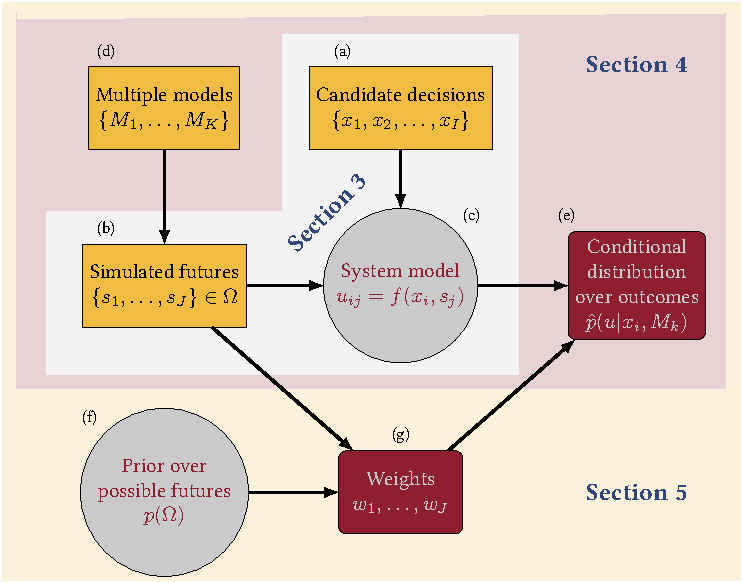
\includegraphics[width=\textwidth]{bayes-rdm.pdf}
  \caption{
    Outline of the proposed decision-analytic framework.
    In \cref{sec:analysis-explore} we use an exploratory framework to quantify the performance \DIFdelbeginFL \DIFdelFL{(c) }\DIFdelendFL of candidate decisions \DIFdelbeginFL \DIFdelFL{(a) }\DIFdelendFL under a large ensemble of possible futures\DIFdelbeginFL \DIFdelFL{(b)}\DIFdelendFL .
    In \cref{sec:analysis-condition} we illustrate the ``multiple PDF problem'' by creating probability distributions over outcomes \DIFdelbeginFL \DIFdelFL{(e) }\DIFdelendFL that are conditional upon specific \DIFdelbeginFL \DIFdelFL{models describing the likelihood of different futures (d)}\DIFdelendFL \DIFaddbeginFL \DIFaddFL{probabilistic scenarios}\DIFaddendFL .
    In our case study, these \DIFdelbeginFL \DIFdelFL{are \mbox{%DIFAUXCMD
        \gls{rcp} }\hskip0pt%DIFAUXCMD
    }\DIFdelendFL scenarios \DIFdelbeginFL \DIFdelFL{and }\DIFdelendFL \DIFaddbeginFL \DIFaddFL{correspond to combinations of emissions pathways with }\DIFaddendFL physical models \DIFdelbeginFL \DIFdelFL{of }\DIFdelendFL \DIFaddbeginFL \DIFaddFL{for }\DIFaddendFL sea level rise.
    \DIFdelbeginFL \DIFdelFL{Finally }\DIFdelendFL \DIFaddbeginFL \DIFaddFL{Then }\DIFaddendFL in \cref{sec:analysis-synthesize} we \DIFdelbeginFL \DIFdelFL{propose a subjective Bayesian framework }\DIFdelendFL \DIFaddbeginFL \DIFaddFL{describe the need }\DIFaddendFL for synthesizing \DIFaddbeginFL \DIFaddFL{insight }\DIFaddendFL across \DIFdelbeginFL \DIFdelFL{deep uncertainties by re-weighting sampled futures (f)}\DIFdelendFL \DIFaddbeginFL \DIFaddFL{scenarios}\DIFaddendFL .
    \DIFaddbeginFL \DIFaddFL{Finally in \mbox{%DIFAUXCMD
        \cref{sec:reweighting} }\hskip0pt%DIFAUXCMD
      we provide a formal framework for doing so.
    }\DIFaddendFL }\label{fig:flowchart}
\end{figure}

\subsection{\DIFdelbegin \DIFdel{Explore}\DIFdelend \DIFaddbegin \DIFadd{Exploratory modeling}\DIFaddend }\label{sec:analysis-explore}

A first analytical step is to use the model in an ``exploratory'' mode.
Exploratory modeling \DIFdelbegin \DIFdel{is averse to }\DIFdelend \DIFaddbegin \DIFadd{strives to avoid }\DIFaddend making explicit assumptions about the likelihood of different \glspl{sow} and instead seeks to generate new knowledge \cite{bankes:1993} by systematically exploring a large number of possible futures, emphasizing interactions between different uncertainties \cite{reed_msdbook:2022}.
Exploratory modeling is often paired with analyses that identify relevant scenarios  \cite{lamontagne_discovery:2018,groves_scenarios:2007} or summarize a system's response to forcing \cite{Poff:2015jn,Steinschneider:2015kk,sriver_sealevel:2018}.
Despite the aversion to strong assumptions about the likelihood of different futures, subjective modeling decisions such as the choice of system model, the set of candidate decisions, the criteria used to assess outcomes, and the choice of how to sample \glspl{sow} can strongly influence results \DIFdelbegin \DIFdel{\mbox{%DIFAUXCMD
    \cite{quinn_exploratory:2020}}\hskip0pt%DIFAUXCMD
}\DIFdelend \DIFaddbegin \DIFadd{\mbox{%DIFAUXCMD
    \cite{quinn_exploratory:2020,quinn_rivalframings:2017,moallemi_decisionsupport:2020}}\hskip0pt%DIFAUXCMD
}\DIFaddend .

\subsection{\DIFdelbegin \DIFdel{Condition}\DIFdelend \DIFaddbegin \DIFadd{Scenario-conditional probabilistic analysis}\DIFaddend }\label{sec:analysis-condition}

Although exploratory modeling is a useful framework for understanding systems, there are many questions that it cannot answer.
For example, answering questions like ``what is the 95th percentile of metric $u$ under decision $x$''  or ``\DIFdelbegin \DIFdel{which decision minimizes expected damages'' or ``}\DIFdelend what is the probability of exceeding a critical threshold'' requires \DIFdelbegin \DIFdel{constructing estimators for the }\DIFdelend \DIFaddbegin \DIFadd{an implicit or explicit }\DIFaddend probability distribution over outcomes \cite<see>[for a general discussion]{schneider_scenarios:2002}.

One way to interpret an ensemble of \glspl{sow} is as \DIFdelbegin \DIFdel{\mbox{%DIFAUXCMD
    \gls{iid} }\hskip0pt%DIFAUXCMD
}\DIFdelend \DIFaddbegin {\DIFadd{iid}} \DIFaddend draws from some \DIFdelbegin \DIFdel{true }\DIFdelend \DIFaddbegin \DIFadd{probabilistic }\DIFaddend data generating process.
This commonly arises when a single deep uncertainty (\eg, an emissions pathway) is used as an input for a \DIFdelbegin \DIFdel{fully probabilistic model; we call this scenario-conditional probabilistic analysis.
  We add this concept to our framework with }\DIFdelend \DIFaddbegin \DIFadd{stochastic model.
  We illustrate this concept in }\DIFaddend boxes (d) and (e) of \cref{fig:flowchart}, denoting the particular scenario \DIFdelbegin \DIFdel{(}%DIFDELCMD < \ie%%%
\DIFdel{, the assumed input) }\DIFdelend $M_k$.
\DIFdelbegin \DIFdel{If the \mbox{%DIFAUXCMD
    \glspl{sow} }\hskip0pt%DIFAUXCMD
  are drawn \mbox{%DIFAUXCMD
    \gls{iid} }\hskip0pt%DIFAUXCMD
}\DIFdelend \DIFaddbegin \DIFadd{By treating the \mbox{%DIFAUXCMD
    \glspl{sow} }\hskip0pt%DIFAUXCMD
  as \mbox{%DIFAUXCMD
    \gls{iid} }\hskip0pt%DIFAUXCMD
  draws }\DIFaddend from $M_k$, the set of outcomes $u_{i, j}$ can be interpreted as \gls{iid} draws from the conditional distribution over outcomes, $p(u | x_i, M_k)$\DIFdelbegin \DIFdel{, allowing estimation of descriptive metrics.
  This approach allows for }\DIFdelend \DIFaddbegin \DIFadd{.
  This ``scenario-conditional'' probabilistic interpretation of \mbox{%DIFAUXCMD
    \glspl{sow} }\hskip0pt%DIFAUXCMD
  allows for fully probabilistic }\DIFaddend quantification of uncertainty \DIFdelbegin \emph{\DIFdel{within}} %DIFAUXCMD
\DIFdel{models of deeply uncertain processes, but can only }\DIFdelend \DIFaddbegin \DIFadd{and optimization, conditional on a particular scenario.
  For example, \mbox{%DIFAUXCMD
    \citeA{fletcher_learning:2019} }\hskip0pt%DIFAUXCMD
  uses stochastic dynamic programming to quantify the value of flexibility in water resources planning.
  However, only a single \mbox{%DIFAUXCMD
    \gls{rcp} }\hskip0pt%DIFAUXCMD
  scenario (\mbox{%DIFAUXCMD
    \gls{rcp} }\hskip0pt%DIFAUXCMD
  8.5) is used.
  While the analysis could be repeated for other \mbox{%DIFAUXCMD
    \gls{rcp} }\hskip0pt%DIFAUXCMD
  scenarios, the scenario-conditional analysis framework only }\DIFaddend qualitatively characterize uncertainty \emph{between} \DIFdelbegin \DIFdel{models }\DIFdelend \DIFaddbegin \DIFadd{scenarios }\DIFaddend \cite{wong_nola:2017,ruckert_coastal:2019,sharma_rcp:2021}.

We can also \DIFdelbegin \DIFdel{use this approach to understand }\DIFdelend \DIFaddbegin \DIFadd{characterize }\DIFaddend \gls{dmdu} methods that sample a set of parameters from fixed ranges \DIFaddbegin \DIFadd{as scenario-conditional analyses}\DIFaddend .
For example, \citeA{sriver_sealevel:2018} sample parameters describing the rate of \gls{slr} across a range of values to inform coastal adaptation.
Similarly, \citeA{trindade_waterpathways:2020} checks the performance of candidate decisions against an ensemble of synthetic time series of streamflow, water demand, and other parameters by sampling parameters that transform the available data over a plausible range\DIFdelbegin \DIFdel{\mbox{%DIFAUXCMD
    \cite<\ie, robustness metrics; see>[for details]{mcphail_robustness:2019,herman:2015}}\hskip0pt%DIFAUXCMD
  .
  Since sampling over a range is equivalent to sampling from a Uniform distribution, this assumption is equivalent to assuming the true inputs to come }\DIFdelend \DIFaddbegin \DIFadd{.
  Analyses that use this methodology are implicitly assuming a single probabilistic model in which different variables are drawn }\DIFaddend from independent Uniform distributions\DIFdelbegin \DIFdel{(one for each parameter) bounded by the plausible range.
}%DIFDELCMD < 

%DIFDELCMD < %%%
\DIFdelend \DIFaddbegin \DIFadd{.
  Many limitations of Uniform and other noninformative priors have been documented in the literature, including (i) that they can induce unrealistic implicit priors over functions of parameters and (ii) results are sensitive to the parameterization of a given process \mbox{%DIFAUXCMD
    \cite{seaman_noninformative:2012}}\hskip0pt%DIFAUXCMD
  .
  Yet while replacing Uniform distributions with alternatives such as maximum-entropy distributions can address some of these challenges \mbox{%DIFAUXCMD
    \cite<\eg,>{gupta_prior:2022}}\hskip0pt%DIFAUXCMD
  , subjective modeling choices remain necessary.
}\DIFaddend Our primary concern \DIFaddbegin \DIFadd{here }\DIFaddend is not that \DIFdelbegin \DIFdel{subjective assumptions about the likelihood of different futures }\DIFdelend \DIFaddbegin \DIFadd{these subjective modeling assumptions }\DIFaddend are wrong -- this is, almost surely, inevitable -- but that when these assumptions are opaque and presented without critique or validation \DIFaddbegin \DIFadd{\mbox{%DIFAUXCMD
    \cite<see>[regarding the importance of iterative critique]{gelman_workflow:2020} }\hskip0pt%DIFAUXCMD
}\DIFaddend they may lead to inscrutable decision processes and \DIFdelbegin \DIFdel{sub-optimal }\DIFdelend \DIFaddbegin \DIFadd{poor }\DIFaddend decisions.

\subsection{\DIFdelbegin \DIFdel{Synthesize}\DIFdelend \DIFaddbegin \DIFadd{Synthesizing deep uncertainties for decision analysis}\DIFaddend }\label{sec:analysis-synthesize}

\DIFdelbegin \DIFdel{As discussed in the previous subsection, estimating the expectation of arbitrary functions under uncertainty is a critical component of decision making under uncertainty.
  If the }\DIFdelend \DIFaddbegin \DIFadd{Scenario-conditional probabilistic analysis allows for uncertainty quantification and optimization, and is valuable in many copntexts.
  However, scenarios are often explicitly provided without probabilities or likelihoods \mbox{%DIFAUXCMD
    \cite<\eg, the \acrlongpl{ssp}>{vanvuuren_conditional:2008}}\hskip0pt%DIFAUXCMD
  .
  Thus, any such analysis is silent on the question of how to combine information across different scenarios.
  We term this the ``multiple \mbox{%DIFAUXCMD
    \gls{pdf} }\hskip0pt%DIFAUXCMD
  problem''.
  Decision making around the multiple \mbox{%DIFAUXCMD
    \gls{pdf} }\hskip0pt%DIFAUXCMD
  problem is susceptible to the cognitive biases that interfere with decision-making under uncertainty more generally \mbox{%DIFAUXCMD
    \cite{tversky_judgment:1974,morgan_uncertainty:1990,srikrishnan_probabilistic:2022}}\hskip0pt%DIFAUXCMD
  .
  For example, while many analyses treat all scenarios as equally likely, this is often inconsistent with available information and can lead to poor decisions and outcomes \mbox{%DIFAUXCMD
    \cite{wigley_equallylikely:2001,ho_scenarios:2019,hausfather_scenarios:2020}}\hskip0pt%DIFAUXCMD
  .
  Other analyses suggest using the worst-case scenario as a conservative measure.
  However, this approach is also problematic, since (i) there are no fundamental limits on what constitutes a worst-case scenario and (ii) improving performance under unlikely worst-case scenarios may lead to substantially impaired performance under more likely scenarios, which may or may not be acceptable to relevant stakeholders.
  There is thus a critical need for synthesizing insights across multiple probabilistic scenarios.
}

\section{\DIFadd{Re-weighting SOWs to synthesize across scenarios}}\label{sec:reweighting}

\DIFadd{In this section we provide a formal method for synthesizing across multiple scenarios to inform climate risk management.
  Our objective is to develop a framework that (i) is conceptually and practically amenable to exploratory modeling; (ii) makes subjective modeling choices explicit and transparent; and (iii) allows decision analysts to estimate a probability distribution over outcomes.
}

\DIFadd{A particular need is to estimate the expectation of functions over \mbox{%DIFAUXCMD
    \glspl{sow} }\hskip0pt%DIFAUXCMD
  (}\ie\DIFadd{, box e in \mbox{%DIFAUXCMD
    \cref{fig:flowchart}}\hskip0pt%DIFAUXCMD
  ).
  If the $J$ }\DIFaddend \glspl{sow} are drawn \gls{iid} from \DIFdelbegin \DIFdel{the true distribution, }\DIFdelend \DIFaddbegin \DIFadd{some distribution that credibly represents the true likelihood of different futures }\DIFaddend then the expected value of \DIFdelbegin \DIFdel{some function$f$, $\mathbb{E}\qty[f(\vb{s})]$}\DIFdelend \DIFaddbegin \DIFadd{such a function}\DIFaddend , \DIFaddbegin \DIFadd{$f(\mathbf{s})$, }\DIFaddend can be readily \DIFdelbegin \DIFdel{estimated as $\frac{1}{N} \sum_{j=1}^N f(\vb{s}_j)$}\DIFdelend \DIFaddbegin \DIFadd{approximated using the Monte Carlo estimate $\mathbb{E}\qty[f(\vb{s})] \approx \frac{1}{N} \sum_{j=1}^N f(\vb{s}_j)$}\DIFaddend .
However, this is often not the case\DIFdelbegin \DIFdel{; for example, a fixed set of simulations may be available for analysis or low-probability but high-impact regions of the parameter space may have been sampled }\DIFdelend \DIFaddbegin \DIFadd{.
  For example, in \mbox{%DIFAUXCMD
    \cref{sec:case-study} }\hskip0pt%DIFAUXCMD
  we will consider decision analysis where the \mbox{%DIFAUXCMD
    \glspl{sow} }\hskip0pt%DIFAUXCMD
  are sampled from multiple physical models and \mbox{%DIFAUXCMD
    \gls{rcp} }\hskip0pt%DIFAUXCMD
  scenarios, considering that not all \mbox{%DIFAUXCMD
    \gls{rcp} }\hskip0pt%DIFAUXCMD
  scenarios are equally likely and that not all physical models are equally skillful}\DIFaddend .
In this case, the formula \DIFdelbegin \DIFdel{must }\DIFdelend \DIFaddbegin \DIFadd{may }\DIFaddend be adjusted to \DIFaddbegin \DIFadd{a weighted Monte Carlo estimate:
}\DIFaddend \begin{equation}
  \mathbb{E}\qty[f(\vb{s})] \approx \DIFdelbegin \DIFdel{\frac{1}{N} }\DIFdelend \sum_{i=j}^N w_j f(\vb{s}_j),
\end{equation}
where \DIFdelbegin \DIFdel{the $w_j$ are suitably chosen weights such that their sum is equal to 1.
}\DIFdelend \DIFaddbegin \DIFadd{$\sum_{j=1}^J w_j = 1$.
}\DIFaddend

The challenge then becomes to suitably estimate the $w_j$.
\DIFdelbegin \DIFdel{Paralleling }\DIFdelend \DIFaddbegin \DIFadd{Many such methods exist; drawing from }\DIFaddend joint probability methods for statistical analysis of tropical cyclones, we \DIFdelbegin \DIFdel{use }\DIFdelend \DIFaddbegin \DIFadd{employ }\DIFaddend a grid-based approach \cite{johnson_clara:2013,resio_probabilities:2007,toro_jpm-os:2010}.
First, we project the \glspl{sow} $\vb{s} \in \Omega$ onto a low-dimensional representation, which we denote $\qty{\psi_1, \psi_2, \ldots, \psi_J} \in \Psi$.
Then, we partition the parameter space into a region corresponding to each \gls{sow} and integrating the \DIFdelbegin \DIFdel{\mbox{%DIFAUXCMD
    \gls{pdf} }\hskip0pt%DIFAUXCMD
  $p_\mathrm{belief}$ }\DIFdelend \DIFaddbegin \DIFadd{probability $p(\psi)$ }\DIFaddend over each region.

\DIFaddbegin \DIFadd{Doing so requires a probabilistic model for this low-dimensional representation of the \mbox{%DIFAUXCMD
    \glspl{sow}}\hskip0pt%DIFAUXCMD
  ,  $p(\psi)$.
  We denote this model $p_\mathrm{belief}$ to emphasize that it represents a subjective belief about the \mbox{%DIFAUXCMD
    \glspl{sow}}\hskip0pt%DIFAUXCMD
  , rather than an objectively verifiable choice.
  In general we do not expect that stakeholders and experts will agree on $p_\mathrm{belief}$ because there is not, even conceptually, an objectively correct choice \mbox{%DIFAUXCMD
    \cite{oreskes_verification:1994,walker_deep:2013}}\hskip0pt%DIFAUXCMD
  .
  However, we posit that since we cannot be ``right,'' it is valuable to maximize the transparency of our implicit probabilistic assumptions, and suggest that writing down an explicit model for $p_\mathrm{belief}$ supports this aim.
  Choices for $p_\mathrm{belief}$ can be drawn from many sources, including expert elicitation or  results of previous analyses.
  These models can be interpreted as prior beliefs about \mbox{%DIFAUXCMD
    \gls{slr} }\hskip0pt%DIFAUXCMD
  that could be incorporated into a Bayesian analysis as additional data is collected in the future, and thus can draw from literature on Bayesian prior selection and prior predictive checks \mbox{%DIFAUXCMD
    \cite{gelman_workflow:2020}}\hskip0pt%DIFAUXCMD
  .
}

\DIFaddend We present here the case where the $\psi_j$ are one-dimensional; extensions to higher dimensions are possible.
We first sort the $\psi_j$  from least to greatest so that $\psi_{j-1} \leq \psi_j$, ($j \neq 1$).
Defining \DIFdelbegin \DIFdel{$F_\mathrm{belief}(s)$ to be the cumulative distribution corresponding to $p_\mathrm{belief}$}\DIFdelend \DIFaddbegin \DIFadd{a cumulative distribution function
  $F_\mathrm{belief} \qty(\psi) = \int_{-\infty}^{\psi} p_\mathrm{belief}(\psi') \dd{\psi'}$}\DIFaddend ,
we calculate weights as
\begin{equation}\label{eq:weights}
  w_j = \DIFdelbegin %DIFDELCMD < \begin{cases}
  %DIFDELCMD <     F_\mathrm{belief}\qty(\frac{1}{2}\qty[\psi_1 + \psi_2])                                                                     & j = 1     \\
  %DIFDELCMD <     F_\mathrm{belief}\qty(\frac{1}{2}\qty[\psi_{j} + \psi_{j+1}]) - F_\mathrm{belief}\qty(\frac{1}{2}\qty[\psi_{j-1} + \psi_j]) & 1 < j < J \\
  %DIFDELCMD <     1 - F_\mathrm{belief}\qty(\frac{1}{2}\qty[\psi_{J-1} + \psi_J])                                                             & j = J.
  %DIFDELCMD <   \end{cases}%%%
  \DIFdelend \DIFaddbegin \begin{cases}
    F_\mathrm{belief}\qty(\frac{\psi_1 + \psi_2}{2})                                                              & j = 1     \\
    F_\mathrm{belief}\qty(\frac{\psi_{j} + \psi_{j+1}}{2}) - F_\mathrm{belief}\qty(\frac{\psi_{j-1} + \psi_j}{2}) & 1 < j < J \\
    1 - F_\mathrm{belief}\qty(\frac{\psi_{J-1} + \psi_J}{2})                                                      & j = J.
  \end{cases}\DIFaddend
\end{equation}
This step is illustrated in \cref{fig:grid-sketch}.
\DIFaddbegin \DIFadd{By the definition of cumulative distribution functions, $F_\mathrm{belief}(b) - F_\mathrm{belief}(a) = \int_a^b p_\mathrm{belief}(\psi') \dd{\psi'}$.
}\DIFaddend Diagnostic checks, such as examining the histogram of weights \DIFaddbegin \DIFadd{to }\DIFaddend (not shown), may be \DIFdelbegin \DIFdel{valuable }\DIFdelend \DIFaddbegin \DIFadd{useful }\DIFaddend protections against degeneracy.

\begin{figure}
  \centering
  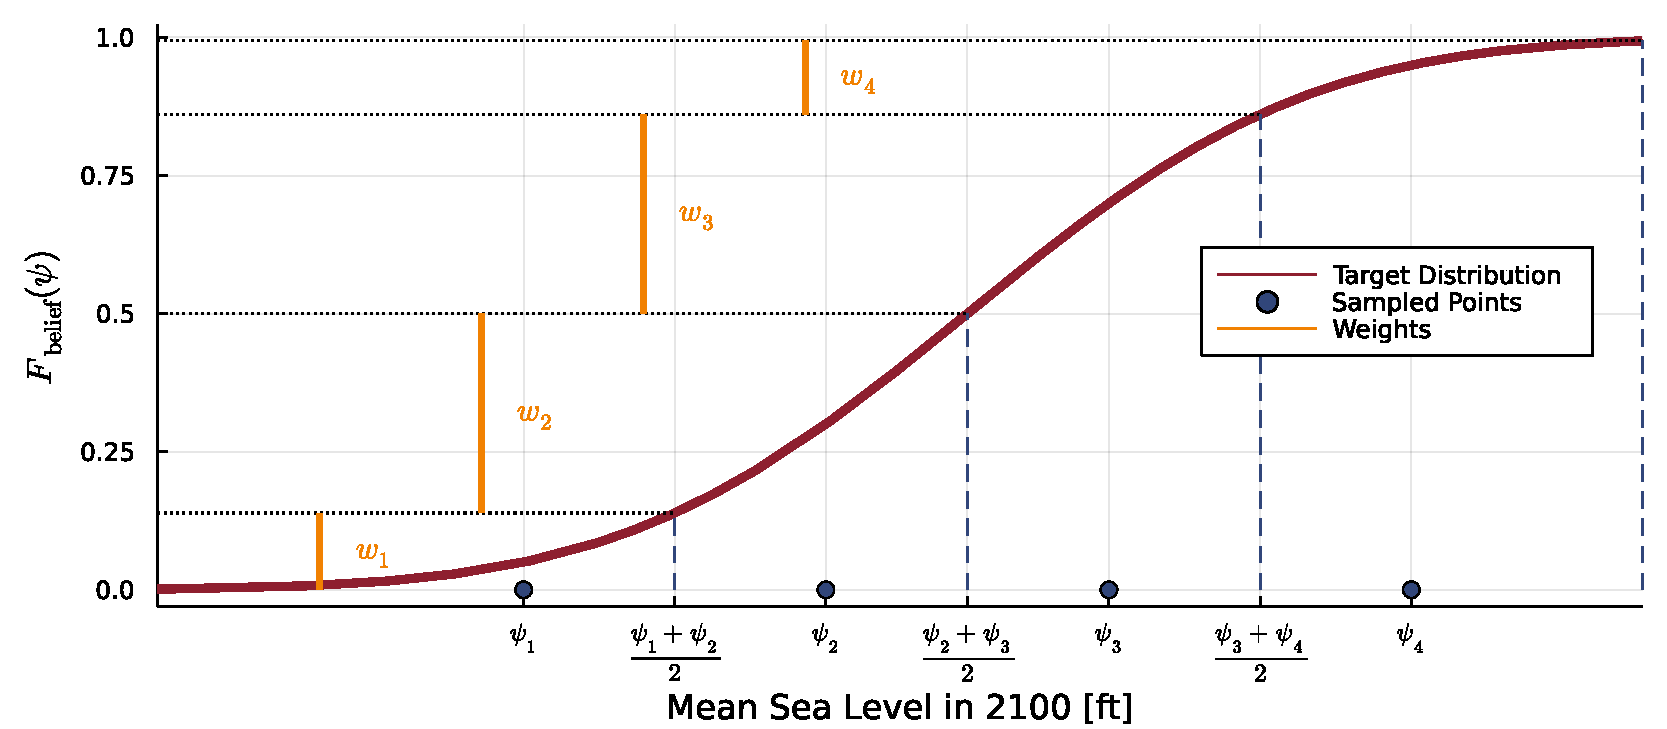
\includegraphics[width=\textwidth]{grid-sketch}
  \caption{
    Schematic of \gls{sow} \DIFdelbeginFL \DIFdelFL{weighting }\DIFdelendFL \DIFaddbeginFL \DIFaddFL{re-weighting }\DIFaddendFL scheme defined in \cref{eq:weights}.
    This method is illustrated for a hypothetical target distribution (dark red line) and $J=4$ samples $\psi_1, \psi_2, \psi_3, \psi_4$ (blue dots).
    As shown in \cref{eq:weights}, the weights $w_j$ (orange vertical lines) are calculated based on the cumulative distribution function of the target distribution at the halfway points $\frac{1}{2}\qty[\psi_j+\psi_{j+1}]$ (vertical dashed lines).
  }\label{fig:grid-sketch}
\end{figure}

The aim of this re-weighting framework is to integrate an ensemble of \glspl{sow} used for exploratory modeling into formal decision analysis, even when the \glspl{sow} deliberately over- or under-sample some regions of the parameter space.
As in \cref{sec:analysis-condition}, we must condition on a model: where the analysis of \cref{sec:analysis-condition} conditions upon deep uncertainties, the approach outlined in this subsection synthesizes across them.
\DIFdelbegin \DIFdel{We reiterate that stakeholders and experts will not, in general, agree on }\DIFdelend \DIFaddbegin \DIFadd{Considering multiple probabilistic models for }\DIFaddend $p_\mathrm{belief}$ \DIFdelbegin \DIFdel{because there is not, even conceptually, an objectively correct choice \mbox{%DIFAUXCMD
    \cite{oreskes_verification:1994,walker_deep:2013}}\hskip0pt%DIFAUXCMD
  .
  However, we posit that since we cannot be ``right, '' it is valuable to maximize the transparency of our implicit probabilistic assumptions, and suggest that writing down an explicit model for }\DIFdelend \DIFaddbegin \DIFadd{can also be useful for understanding the sensitivity of the decision to the choice of $p_\mathrm{belief}$.
  Further, the sensitivity, or lack thereof, of different objectives to the choice of }\DIFaddend $p_\mathrm{belief}$ \DIFdelbegin \DIFdel{supports this aim}\DIFdelend \DIFaddbegin \DIFadd{may be useful for identifying future research needs}\DIFaddend .

\section{Demonstrating the concept with a case study}\label{sec:case-study}

To illustrate the proposed decision analytic framework, we model a one-time decision of whether to elevate a house, and if so by how much (\cref{fig:xlrm}).
Following the approach outlined in \citeA{zarekarizi_suboptimal:2020}, we focus on a case study of a \emph{hypothetical} house in Norfolk, VA.
For interpretability, we focus on deep uncertainty in \gls{msl} and \DIFdelbegin \DIFdel{approximate }\DIFdelend \DIFaddbegin \DIFadd{treat storm surge and }\DIFaddend other model parameters as shallow uncertainties as shown in \cref{tab:uncertainties}.
We use the notation developed in the previous section to describe the case study.
Specifically,
\begin{enumerate}
  \item The decision vector $\vb{x}$ is comprised of discrete possible house heightenings ($\Delta h$); we consider $\Delta h = \qty{\SI{0}{ft}, \SI{0.25}{ft}, \ldots, \SI{12}{ft}}$.
  \item The \glspl{sow} describe annual time series of \gls{msl} over the $T=70$ year house lifetime so $\vb{s} \in \mathbb{R}^T$
  \item The system model $f$ quantifies up-front costs (the cost of elevating) and lifetime expected damages (the structural cost of experiencing floods), given a decision $x_i$ and \gls{sow} $s_j$, by integrating economic and engineering damage models over a probability distribution for storm surge. We elaborate upon these metrics in \cref{sec:case-metrics}.
\end{enumerate}
In the remainder of this section we describe data sources and treatment of \gls{slr} (\cref{sec:case-slr}), storm surge (\cref{sec:case-surge}), damages and metrics (\cref{sec:case-metrics}), and finally the subjective \DIFdelbegin \DIFdel{priors }\DIFdelend \DIFaddbegin \DIFadd{probabilistic models }\DIFaddend $p_\mathrm{belief}$ used to apply the re-weighting method described in \cref{sec:analysis-synthesize} to this case study (\cref{sec:case-priors}).

\begin{table}
  \centering
  \caption{
    Summary of parameters, their notation, and how their uncertainty is represented.
    Symbols describing the decision-analytic framework are described in \cref{fig:flowchart}.
  }\label{tab:uncertainties}
  \footnotesize
  \begin{tabular}{p{1.25in} p{0.75in} p{3in}}
    \toprule
    Name                 & Symbol            & Uncertainty                                                                          \\
    \midrule
    \Gls{msl}            & $\overline{y}(t)$ & Deeply uncertain: four physical models $\times$ four \acrshort{rcp} scenarios        \\
    Storm surge          & $y'(t)$           & Probabilistic: Bayesian inference on a stationary \acrshort{gev} model               \\
    Annual maximum flood & $y(t)$            & Deterministic: $y(t)=\overline{y}(t)+y'(t)$                                          \\
    Discount rate        & $\rho$            & Determinitic: 2.5\% per year                                                         \\
    Depth-damage         & $D(h-y)$          & Deterministic: based on HAZUS model \cite<see>[]{zarekarizi_suboptimal:2020}         \\
    Elevation cost       & $C(\Delta h)$     & Deterministic: a piecewise linear model following \citeA{zarekarizi_suboptimal:2020} \\
    Initial height       & $h_0$             & Deterministic: \SI{1}{ft} below the \gls{bfe}, unless otherwise noted                \\
    House floor area     & --                & Deterministic: \SI{1500}{ft^2}                                                       \\
    Structural value     & --                & Deterministic: \usd{200000}                                                          \\
    House lifespan       & $T$               & Deterministic: 70 years                                                              \\
    \bottomrule
  \end{tabular}
\end{table}

\begin{figure}
  \centering
  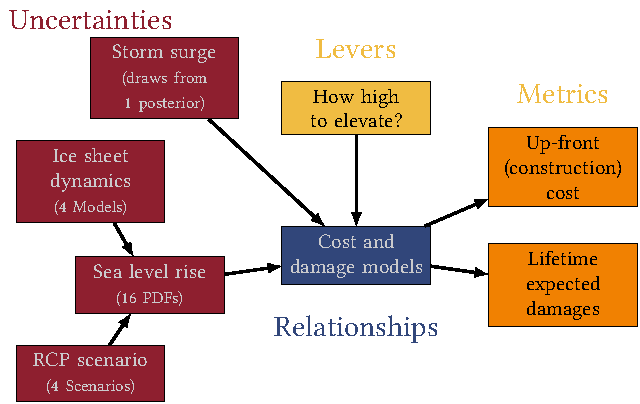
\includegraphics[width=\textwidth]{xlrm.pdf}
  \caption{
    Conceptual diagram of the considered example.
    A \acrfull{sow} consists of a description of the uncertain factors (red).
    We model a problem with a single lever (yellow), which is how high to elevate a house ($\Delta h$).
    For each \acrshort{sow} (red) and each value of $\Delta h$, the system model (blue) is used to calculate performance metrics (gray).
    We also compute a third metric, expected lifetime costs, which is the sum of up-front costs and lifetime expected damages.
  }\label{fig:xlrm}
\end{figure}

\subsection{\Glsentrylong{slr}}\label{sec:case-slr}

We analyze simulations of \gls{msl} at Sewells Point, VA from four probabilistic physical models using data published in \citeA{ruckert_coastal:2019}.
The four models considered are (i) the BRICK model (version 0.2) with slow (``BRICK Slow'') and (ii) fast (``BRICK Fast'') ice sheet dynamics \cite{wong_brick0.2:2017}, (iii) the \citeA{kopp_probabilistic:2014} model (``K14''), and (iv) the \citeA{deconto_antarctica:2016} model (``DP16'').
The \citeA{kopp_probabilistic:2014} and \citeA{deconto_antarctica:2016} models have a ten year time step, which we linearly interpolate onto a one year time step for consistency.
\DIFdelbegin \DIFdel{These four models represent physical processes, particularly of ice sheet dynamics, in different ways.
  The differences in these models leading to diverging estimates of how \mbox{%DIFAUXCMD
    \gls{msl} }\hskip0pt%DIFAUXCMD
  responds to temperature.
  For a discussion of these model outputs we refer the reader to \mbox{%DIFAUXCMD
    \citeA{ruckert_coastal:2019}}\hskip0pt%DIFAUXCMD
  .
}%DIFDELCMD < 

%DIFDELCMD < %%%
\DIFdelend Estimates of nonstationary \gls{msl} also depend on anthropogenic forcing, which is itself deeply uncertain \cite{ho_scenarios:2019,srikrishnan_probabilistic:2022}.
To sample this uncertainty, we use simulations from each physical model under four \gls{rcp} scenarios, yielding sixteen time-varying \DIFdelbegin \DIFdel{distributions }\DIFdelend \DIFaddbegin \DIFadd{probabilistic scenarios }\DIFaddend of \gls{msl}.

\begin{figure}
  \centering
  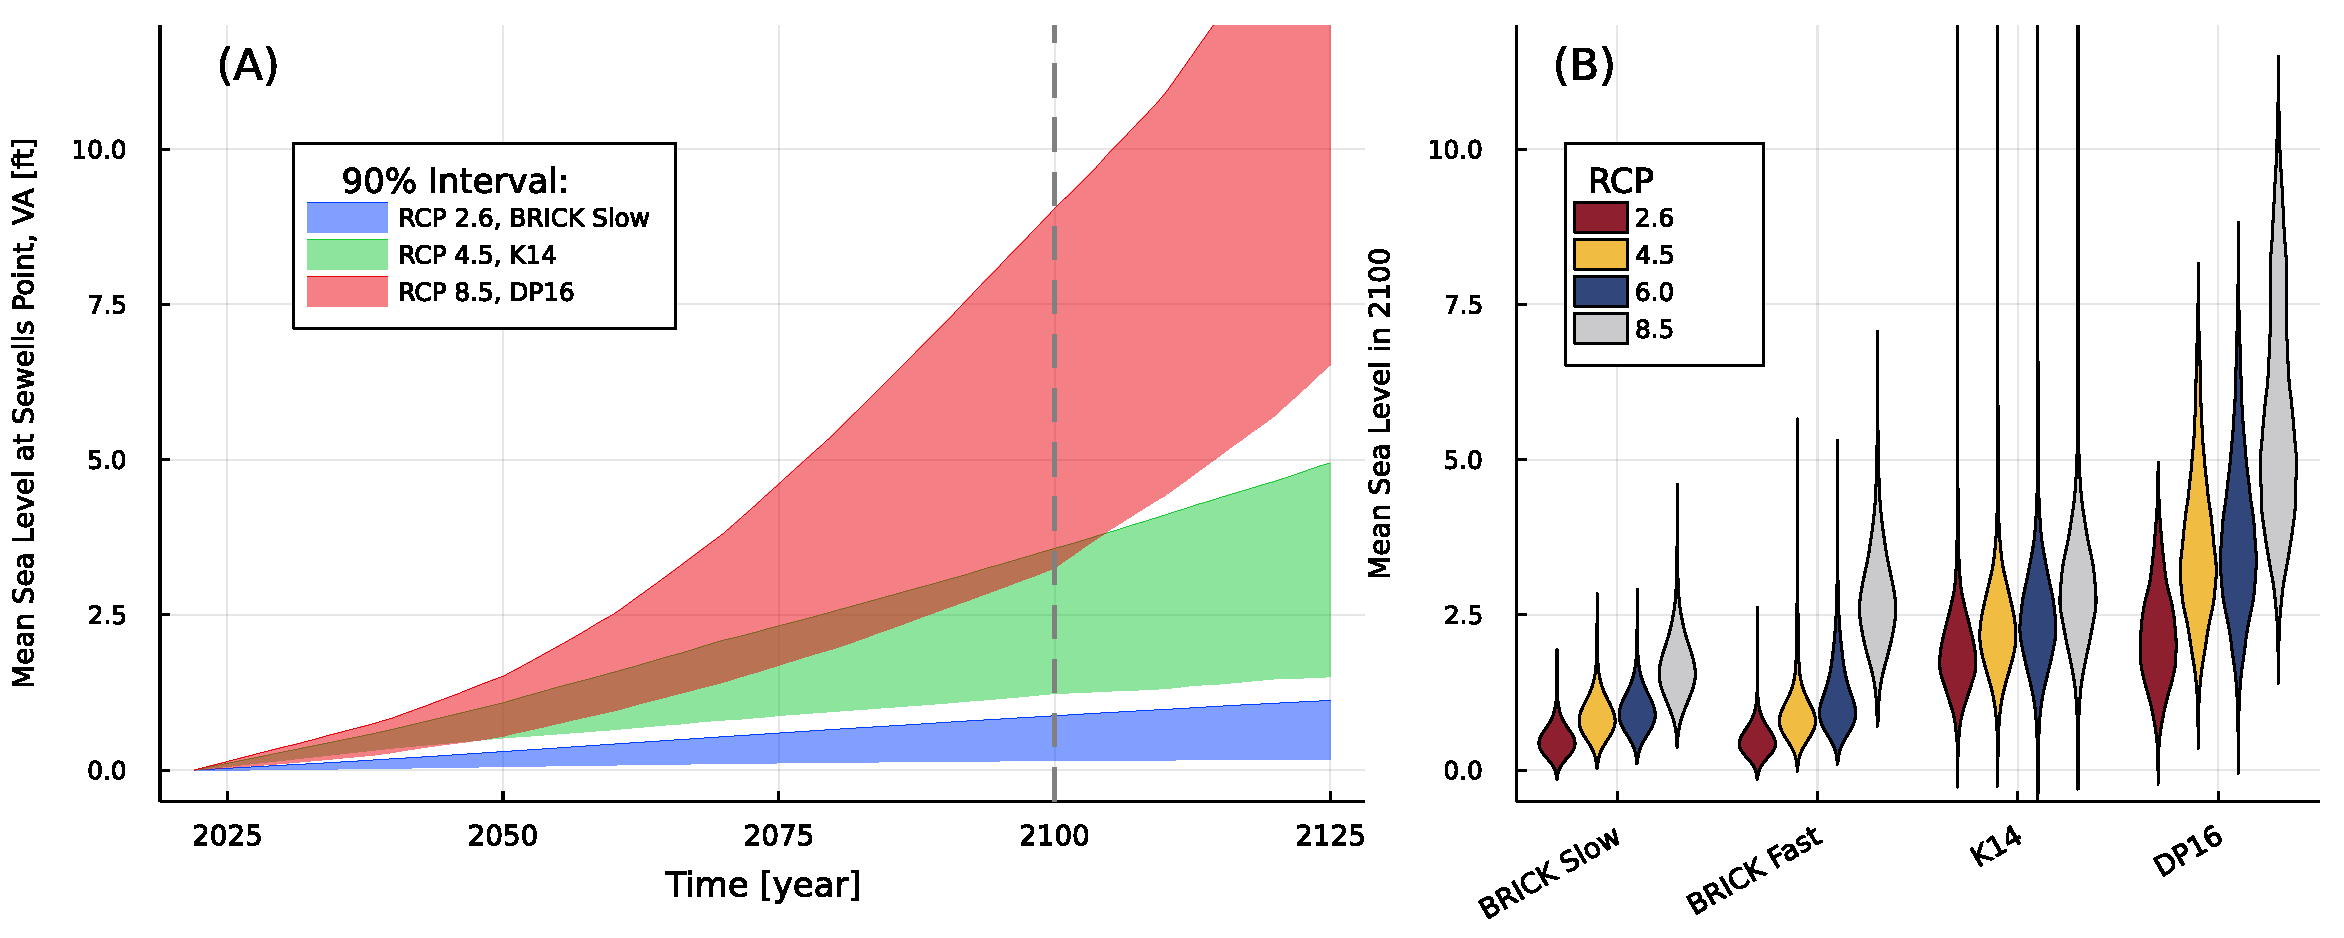
\includegraphics[width=\textwidth]{lsl-evolution}
  \caption{
    Projections of future mean sea level depend strongly on the choices of physical model and forcing.
    (A): 90\% confidence intervals for mean sea level at Sewells Point, VA as a function of time for a representative subset of three probabilistic models (out of sixteen).
    (B): probability distribution of \gls{msl} at Sewells Point, VA in the year 2100 for each probabilistic model considered.
  }\label{fig:lsl-evolution}
\end{figure}

The choices of physical model and \gls{rcp} scenario jointly determine future \gls{msl} $p(\overline{y}|t)$.
\Cref{fig:lsl-evolution}(a) shows the time-varying 90\% credible intervals of \gls{msl} for three representative models.
The divergence between the the best-case (blue) and worst-case (red) models is small in the early 21st century and increases rapidly thereafter.
\Cref{fig:lsl-evolution}(b) shows the \glspl{pdf} of mean sea level in 2100 (dashed vertical line in panel (a)) under each of the sixteen \DIFdelbegin \DIFdel{models considered.
}\DIFdelend \DIFaddbegin \DIFadd{probabilistic scenarios considered.
  The stark differences between different scenarios of \mbox{%DIFAUXCMD
    \gls{slr} }\hskip0pt%DIFAUXCMD
  arise primarily from different representations of Antarctic Ice Sheet contributions to global \mbox{%DIFAUXCMD
    \gls{slr} }\hskip0pt%DIFAUXCMD
  and statistical calibration methodologies.
  For a more detailed discussion we refer the reader to \mbox{%DIFAUXCMD
    \citeA{ruckert_coastal:2019}}\hskip0pt%DIFAUXCMD
  .
}\DIFaddend We return in \cref{sec:results-conditional} to the challenge of decision making \DIFdelbegin \DIFdel{under }\DIFdelend \DIFaddbegin \DIFadd{given }\DIFaddend multiple \glspl{pdf}.

\subsection{Storm surges}\label{sec:case-surge}

Following prior work \cite<\eg,>[]{garner_slrise:2018,sriver_sealevel:2018}, we model annual maximum floods $y(t)$ as the sum of sea level $\overline{y}(t)$, described in the previous subsection, and annual maximum storm surges $y'(t)$, neglecting \DIFdelbegin \DIFdel{hydrodynamic effects}\DIFdelend \DIFaddbegin \DIFadd{any potential hydrodynamic interactions}\DIFaddend .

We use data on storm surge at Sewells Point, VA (gauge 8638610) from the \gls{noaa} tides and currents data archive \cite{noaa_tidesandcurrents:2022}.
Hourly recordings of water level are available from 1928 to the present; we use data from the period January 1, 1928 to December 31, 2021.
For each calendar year we first remove the annual mean, then calculate the maximum water level.
We refer this time series of annual maximum storm surges as $y'(t)$.
We display this time series of annual maxima storm surges in \cref{fig:surge-obs-return}(a).
The largest recorded surge was the Chesapeake-Potomac hurricane of 1933, which caused a surge of over \SI{7}{ft} at this gauge, but other hurricanes and Nor'easters have caused surges above \SI{6}{ft}.

\begin{figure}
  \centering
  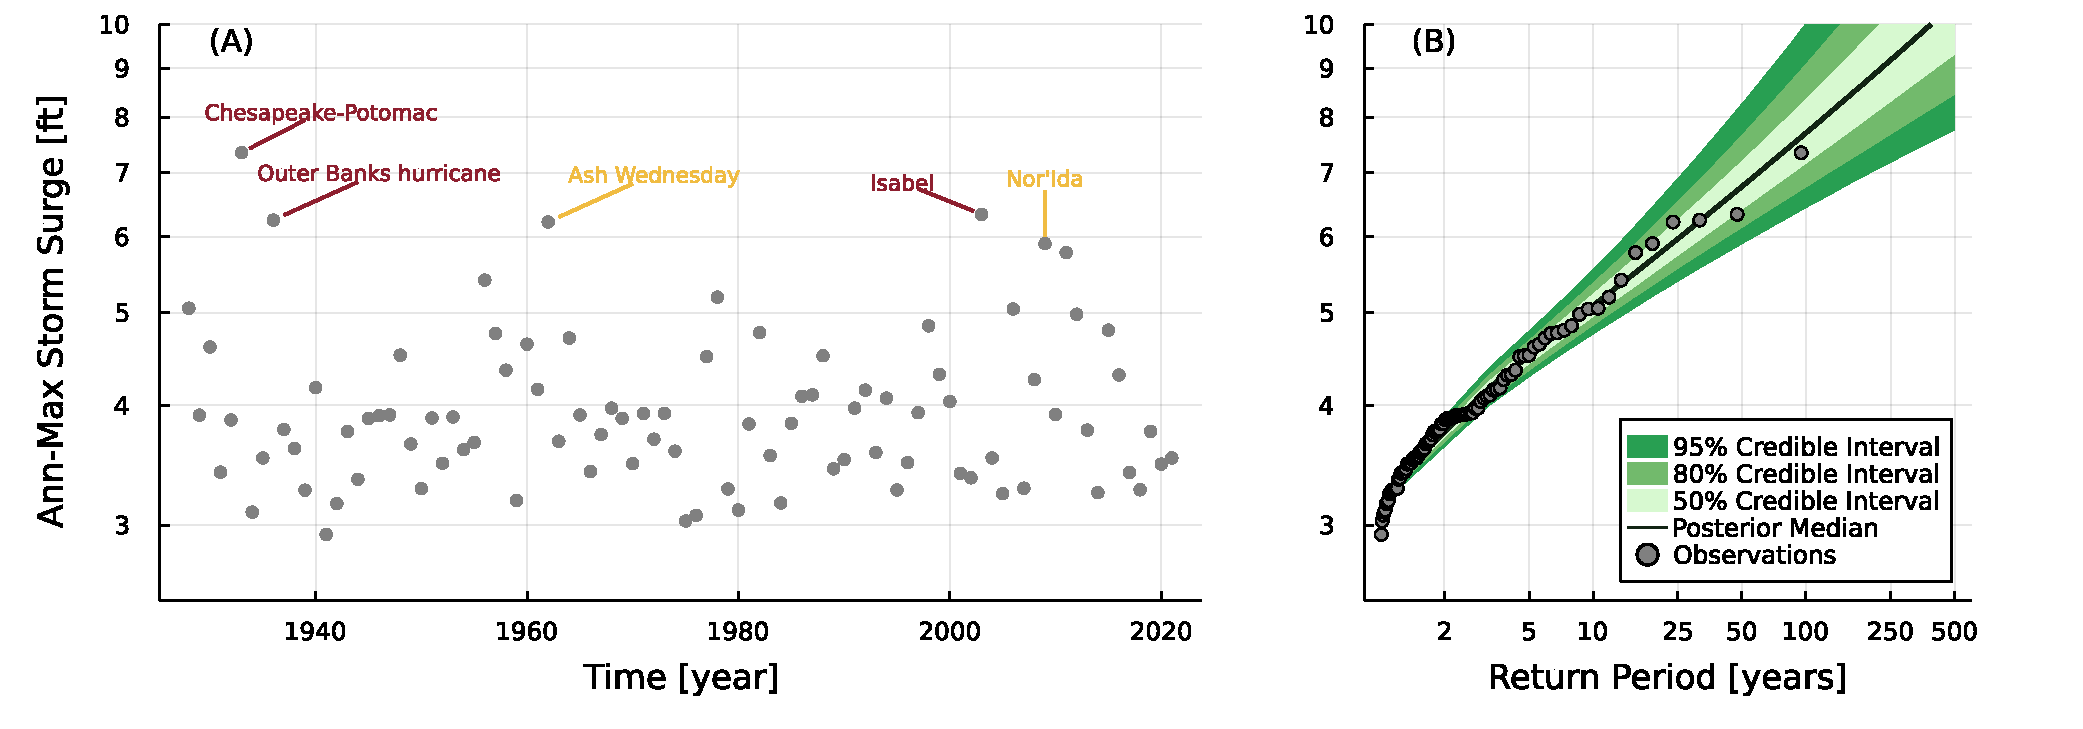
\includegraphics[width=\textwidth]{surge-obs-return}
  \caption{
    Annual maximum storm surges (after subtracting \acrlong{msl}) at Sewells Point, VA from the freely available NOAA tides and currents data archive \protect\cite{noaa_tidesandcurrents:2022}.
    (A):
    time series of historic storms.
    Red (yellow) arrows denote notable tropical cyclones (Nor'easters).
    (B):
    return periods.
    Dots indicate observed values; their $x$-value is their plotting position using the Weibull formula (eq.~\DIFdelbeginFL \DIFdelFL{\ref{eq:weibull}}\DIFdelendFL \DIFaddbeginFL \DIFaddFL{S5}\DIFaddendFL ).
    Gray lines show the 50, 80, and 95\% posterior confidence intervals from the Bayesian \gls{gev} fit (\cref{sec:case-surge}).
  }\label{fig:surge-obs-return}
\end{figure}

We model future storm surge using a stationary \gls{gev} model:
\begin{equation}\label{eq:surge-model}
  y'(t) \sim \text{GEV}\qty(\mu, \sigma, \xi),
\end{equation}
where $y'(t)$ is the storm surge (above \gls{msl}) in year $t$ and a \gls{gev} distribution with location, shape, and scale parameters $\mu$, $\sigma$, and $\xi$, respectively, has the probability density function given in \DIFdelbegin \DIFdel{\mbox{%DIFAUXCMD
    \cref{eq:gev-dist}}\hskip0pt%DIFAUXCMD
  .}\DIFdelend \DIFaddbegin \DIFadd{eq.~(S1).
}\DIFaddend This model assumes stationarity, neglecting any potential time dependence.

Our approach to model assessment is based on the concept of principled workflow design for model building and checking \cite<see>[for details]{gelman_workflow:2020}.
One model choice, analogous to the choice of statistical distribution or the assumption of stationarity, is the choice of how to represent prior information.
We include two forms of prior information.
First, we constrain the shape parameter to be positive, $\xi > 0$, to reflect knowledge about the support of $y'$, which for a variable distributed according to \DIFdelbegin \DIFdel{\mbox{%DIFAUXCMD
    \cref{eq:gev-dist} }\hskip0pt%DIFAUXCMD
}\DIFdelend \DIFaddbegin \DIFadd{eq.~S1 }\DIFaddend is:
\begin{equation*}
  \mathrm{supp}~ y' =
  \begin{cases}
    \xi < 0: & y' \in \qty(-\infty,~ \mu - \nicefrac{\sigma}{\xi}) \\
    \xi > 0: & y' \in \qty(\mu-\nicefrac{\sigma}{\xi},~ \infty).
  \end{cases}
\end{equation*}
Since storm surges cannot be negative, only the latter is physically defensible, justifying our choice to constrain the shape parameter to be positive.
Second, we add weakly informative priors.
Rather than applying prior information directly over the joint distribution of the parameters $\qty{\mu,\sigma,\xi}$, we instead apply a prior over extreme quantiles of the distribution, as in \citeA{coles_evd:1996}.
Specifically, we apply Inverse Gamma priors over the 2, 10, 100, and 500 year return levels, with means of \SIlist{4;6;10;15}{ft} and standard deviations of \SIlist{1.5;1.75;2.25;2.75}{ft}, respectively.
The parameters of the Inverse Gamma distribution can be calculated from these moments (see eq.~\DIFdelbegin \DIFdel{\ref{eq:inv-gamma-params}}\DIFdelend \DIFaddbegin \DIFadd{S3}\DIFaddend ).
These means and standard deviations were chosen to represent plausible physical ranges (\DIFdelbegin \DIFdel{\mbox{%DIFAUXCMD
    \cref{fig:surge-gev-priors}}\hskip0pt%DIFAUXCMD
}\DIFdelend \DIFaddbegin \DIFadd{fig.~S4}\DIFaddend ).

For inference, we draw \num{10000} samples from the posterior distribution $p(\mu,\sigma,\xi | y')$ using Hamiltonian Markov Chain Monte Carlo \cite{betancourt_hamiltonian:2018,hoffman_nuts:2011} implemented in the Turing package of the Julia programming language \cite{perkel_julia:2019,ge_turing:2018,tarek_dynamicppl:2020,besancon_distributions.jl:2021,bezanson_julia:2012}.
Diagnostics suggest (though cannot guarantee) convergence (see \DIFdelbegin \DIFdel{\mbox{%DIFAUXCMD
    \cref{tab:surge-posterior-mcmc-diagnostics}}\hskip0pt%DIFAUXCMD
}\DIFdelend \DIFaddbegin \DIFadd{table S1}\DIFaddend ).
We evaluate the model's fit using posterior predictive checks \cite<see>[section 2.4 and references therein]{gelman_workflow:2020}.
Using the lag 1 and 2 partial autocorrelations, sample maximum, sample minimum, sample median, and Mann-Kendall test value as Bayesian test statistics, we find that draws from the posterior predictive distribution match the observed test statistics credibly (\DIFdelbegin \DIFdel{\mbox{%DIFAUXCMD
    \cref{fig:surge-test-statistics}}\hskip0pt%DIFAUXCMD
}\DIFdelend \DIFaddbegin \DIFadd{fig.~S9}\DIFaddend ) although panels (a) and (b) suggest the possibility of temporal structure not captured by our stationary \gls{iid} model.
Future efforts could represent this structure by conditioning the parameters of the distribution on relevant climate indices \cite<as in>[]{wong_surge:2018,farnham_orbrep:2018,farnham_jetstream:2017,ossandon_semibayesian:2021}.

Other model validations lend confidence to the stationary \gls{gev} model selected.
For example, \cref{fig:surge-obs-return}(b) shows the estimated return periods for these storm surges; the estimated return period  (shading) matches the the empirical plotting position (dots) and a positive control test (\DIFdelbegin \DIFdel{\mbox{%DIFAUXCMD
    \cref{fig:surge-synthetic-data-experiment}}\hskip0pt%DIFAUXCMD
}\DIFdelend \DIFaddbegin \DIFadd{fig.~S6}\DIFaddend ) validates the model's ability to recover known parameter values.

\subsection{Damages and metrics}\label{sec:case-metrics}

The system model (``relationships'' in \cref{fig:xlrm}) is comprised of two key pieces.
The first is a fragility model that estimates the expected flood damages for a particular year (``expected annual damages''), given the elevation of the house and the mean sea level for that year.
The second model converts a time series of annual expected damages into lifetime expected damages.

We define expected annual damages in year $t$ as the expectation of the damage function with respect to storm surge.
This expectation depends on the house's height ($h = h_0 + \Delta h$) where $h_0$ is the initial height relative to the gauge and $\Delta h$ is the amount by which the house is elevated.
The expected annual damage is thus
\begin{equation}\label{eq:ead}
  \textrm{EAD}(t) = \mathbb{E}[D \qty(h-\overline{y}(t))] = \int_{y'} p(y') D \qty(h - \qty(\overline{y}(t) + y')) \dd{y'},
\end{equation}
where $D(h-y)$ is a deterministic function specifying damage as a function of flood depth (relative to the house) \DIFaddbegin \DIFadd{and $p(y')$ is the probability density of storm surge}\DIFaddend .
Following \citeA{zarekarizi_suboptimal:2020}, we use the \gls{hazus} depth-damage curves provided by \gls{fema}; this depth-damage relationship is shown in \DIFdelbegin \DIFdel{\mbox{%DIFAUXCMD
    \cref{fig:cost-depth-damage}}\hskip0pt%DIFAUXCMD
  .}\DIFdelend \DIFaddbegin \DIFadd{fig.~S1.
}\DIFaddend For comparison, \DIFdelbegin \DIFdel{\mbox{%DIFAUXCMD
    \cref{fig:cost-depth-damage} }\hskip0pt%DIFAUXCMD
}\DIFdelend \DIFaddbegin \DIFadd{fig.~S1 }\DIFaddend also shows the ``Europa'' depth-damage relationship developed by the Joint Research Center of the European Commission's science and knowledge service \cite{huizinga_depthdamage:2016}.
\DIFaddbegin \DIFadd{Both models show damage increasing with flood depth before reaching an upper limit but differ in the value of the upper limit and the rate at which damages approach it.
}\DIFaddend Although \citeA{zarekarizi_suboptimal:2020} demonstrate that the choice of fragility function is important for informing house elevation, we use only the HAZUS model for simplicity.

The expected annual damage is sometimes calculated by assuming analytically tractable functional forms for the depth-damage relationship and for the  distribution of hazard \cite<\eg,>[]{vandantzig_dike:1956}.
However, the convolution of the HAZUS depth-damage equation with the \gls{gev} posterior does not have a tractable analytic solution.
Instead, we estimate this convolution through a Monte Carlo method (see \DIFdelbegin \DIFdel{\mbox{%DIFAUXCMD
    \cref{sec:alg-ead} }\hskip0pt%DIFAUXCMD
}\DIFdelend \DIFaddbegin \DIFadd{section S1.2 }\DIFaddend for details).
Then, because the expectation in \cref{eq:ead} depends only on $h-\overline{y}(t)$, we calculate expected annual damages for a wide range of possible heights, then use this to train a computationally efficient surrogate model (using linear interpolation; see \DIFdelbegin \DIFdel{\mbox{%DIFAUXCMD
    \cref{sec:surrogate-ead}}\hskip0pt%DIFAUXCMD
}\DIFdelend \DIFaddbegin \DIFadd{section~S1.3}\DIFaddend ).

The second component of the system model converts a time series of $\mathrm{EAD}$ into lifetime expected damages, which we define as the up-front  discounted sum of expected annual damages:
\begin{equation}\label{eq:led}
  \textrm{LED} = \sum_{t=t_i}^{t_f} \gamma^{\qty(t-t_i)} \textrm{EAD}(t),
\end{equation}
where  $\gamma = 1- \rho$ ($\rho$ being the discount rate), the initial time $t_i=2022$, and the end time $t_f = t_i + T - 1$.
Although \citeA{zarekarizi_suboptimal:2020} show that uncertainty in the discount rate is important for decision support, we use a fixed discount rate (see \cref{tab:uncertainties}) for the purposes of this didactic study.
For a more theoretical discussion see \citeA{arrow_discount:2013}.

To assess the performance of a given decision for a specific \gls{sow} (``Metrics'' in \cref{fig:xlrm}), we calculate the following metrics for each decision-\gls{sow} combination:
\begin{enumerate}
  \item ``Up-front cost'' is the cost of elevating a house. Following \citeA{zarekarizi_suboptimal:2020}, we use estimates of construction cost from the Coastal Louisiana Risk Assessment \cite{fischbach_clara:2012}. We normalize this cost by house value; this cost curve is shown in \DIFdelbegin \DIFdel{\mbox{%DIFAUXCMD
            \cref{fig:cost-up-front}}\hskip0pt%DIFAUXCMD
          .}\DIFdelend \DIFaddbegin \DIFadd{fig.~S3 and shows a large up-front cost plus a piecewise linear marginal cost.
        }\DIFaddend \item ``Lifetime expected damages'' is calculated following \cref{eq:led}.
  \item ``Expected lifetime costs'' is the sum of lifetime expected damages and up-front costs.
\end{enumerate}

\subsection{Prior over \glsentrylong{slr}}\label{sec:case-priors}

We construct three probabilistic models for $p_\mathrm{belief}(\psi)$, which represents the amount of \gls{slr} from 2022 to 2100.

We use a Gamma distribution for all three priors, parameterized following \DIFdelbegin \DIFdel{\mbox{%DIFAUXCMD
    \cref{eq:gamma-dist}}\hskip0pt%DIFAUXCMD
  .}\DIFdelend \DIFaddbegin \DIFadd{eq.~(S4).
  The distributions were chosen to be illustrative, rather than to reflect any particular scientific consensus.
  The Gamma distribution is a flexible distribution that can be used to model skewed, lower-bounded distributions, making it an appropriate choice for modeling subjective uncertainty about \mbox{%DIFAUXCMD
    \gls{slr}}\hskip0pt%DIFAUXCMD
  .
}\DIFaddend \Cref{tab:slr-priors} specifies the parameters of these distributions, as well as some quantiles of the distributions.
Their \glspl{pdf} are also plotted in \cref{fig:lsl-priors-weights}(A).

\begin{table}[ht]
  \centering
  \caption{
    Subjective \DIFdelbeginFL \DIFdelFL{priors }\DIFdelendFL \DIFaddbeginFL \DIFaddFL{probability distributions }\DIFaddendFL over \gls{slr} from 2022 to 2100, \ie $p_\mathrm{belief}(\psi)$.
    The name of the distribution, the parameters of the Gamma distribution with shape $\alpha$ and scale $\theta$, and the 2.5, 25, 50, 75, and 97.5th percentiles (values in \si{ft}).
  }\label{tab:slr-priors}
  \begin{tabular}{llllllll}
    \toprule
    Name          & \multicolumn{2}{c}{Parameters} & \multicolumn{5}{c}{Percentiles (in \si{ft})}                                     \\
    \cmidrule(lr){2-3}
    \cmidrule(lr){4-8}
                  & $\alpha$                       & $\theta$                                     & 2.5  & 25.0 & 50.0 & 75.0 & 97.5  \\
    \midrule
    Slow SLR      & 1.75                           & 0.50                                         & 0.08 & 0.39 & 0.72 & 1.19 & 2.57  \\
    Uncertain SLR & 1.75                           & 1.25                                         & 0.21 & 0.98 & 1.79 & 2.97 & 6.41  \\
    Rapid SLR     & 3.50                           & 1.25                                         & 1.06 & 2.66 & 3.97 & 5.65 & 10.01 \\
    \bottomrule
  \end{tabular}
  \DIFdelbeginFL %DIFDELCMD < 

  %DIFDELCMD < %%%
  \DIFdelendFL \end{table}


We developed these priors for didactic purposes, to illustrate a range of possible beliefs.
We can compare them, for example, with analysis published by \gls{noaa}, which project \SIlist{1.94;2.62;4.27;5.25;6.89}{ft} for the low, intermediate, low intermediate, intermediate high, and high scenarios, respectively \cite[table.~2.4]{sweet_slr:2022}.
We can also compare to the analyses of \citeA{sriver_sealevel:2018} which uses a rescaled Beta distribution with bounds of \SIrange{0.83}{8.2}{ft} and a most plausible estimate of \SI{3.1}{ft}.
Our samples bound all of these estimates.

\section{Results and discussion}\label{sec:results}

We illustrate our approach to synthesizing uncertainties by sequentially analyzing the house elevation problem through \DIFdelbegin \DIFdel{the lenses of exploratory modeling (\mbox{%DIFAUXCMD
    \cref{sec:results-exploratory}}\hskip0pt%DIFAUXCMD
  ), scenario-conditional analysis (\mbox{%DIFAUXCMD
    \cref{sec:results-conditional}}\hskip0pt%DIFAUXCMD
  ), and finally the proposed synthesis method (\mbox{%DIFAUXCMD
    \cref{sec:results-synthesis}}\hskip0pt%DIFAUXCMD
  )}\DIFdelend \DIFaddbegin \DIFadd{multiple lenses for \mbox{%DIFAUXCMD
    \gls{dmdu}}\hskip0pt%DIFAUXCMD
  .
  This allows us to demonstrate the advantages and limitations of each approach, and to highlight the value of synthesizing across multiple scenarios}\DIFaddend .

\subsection{Exploratory modeling}\label{sec:results-exploratory}

We begin by using our model in an ``exploratory'' mode with an aim of learning about interactions between system dynamics and decisions.

\begin{figure}
  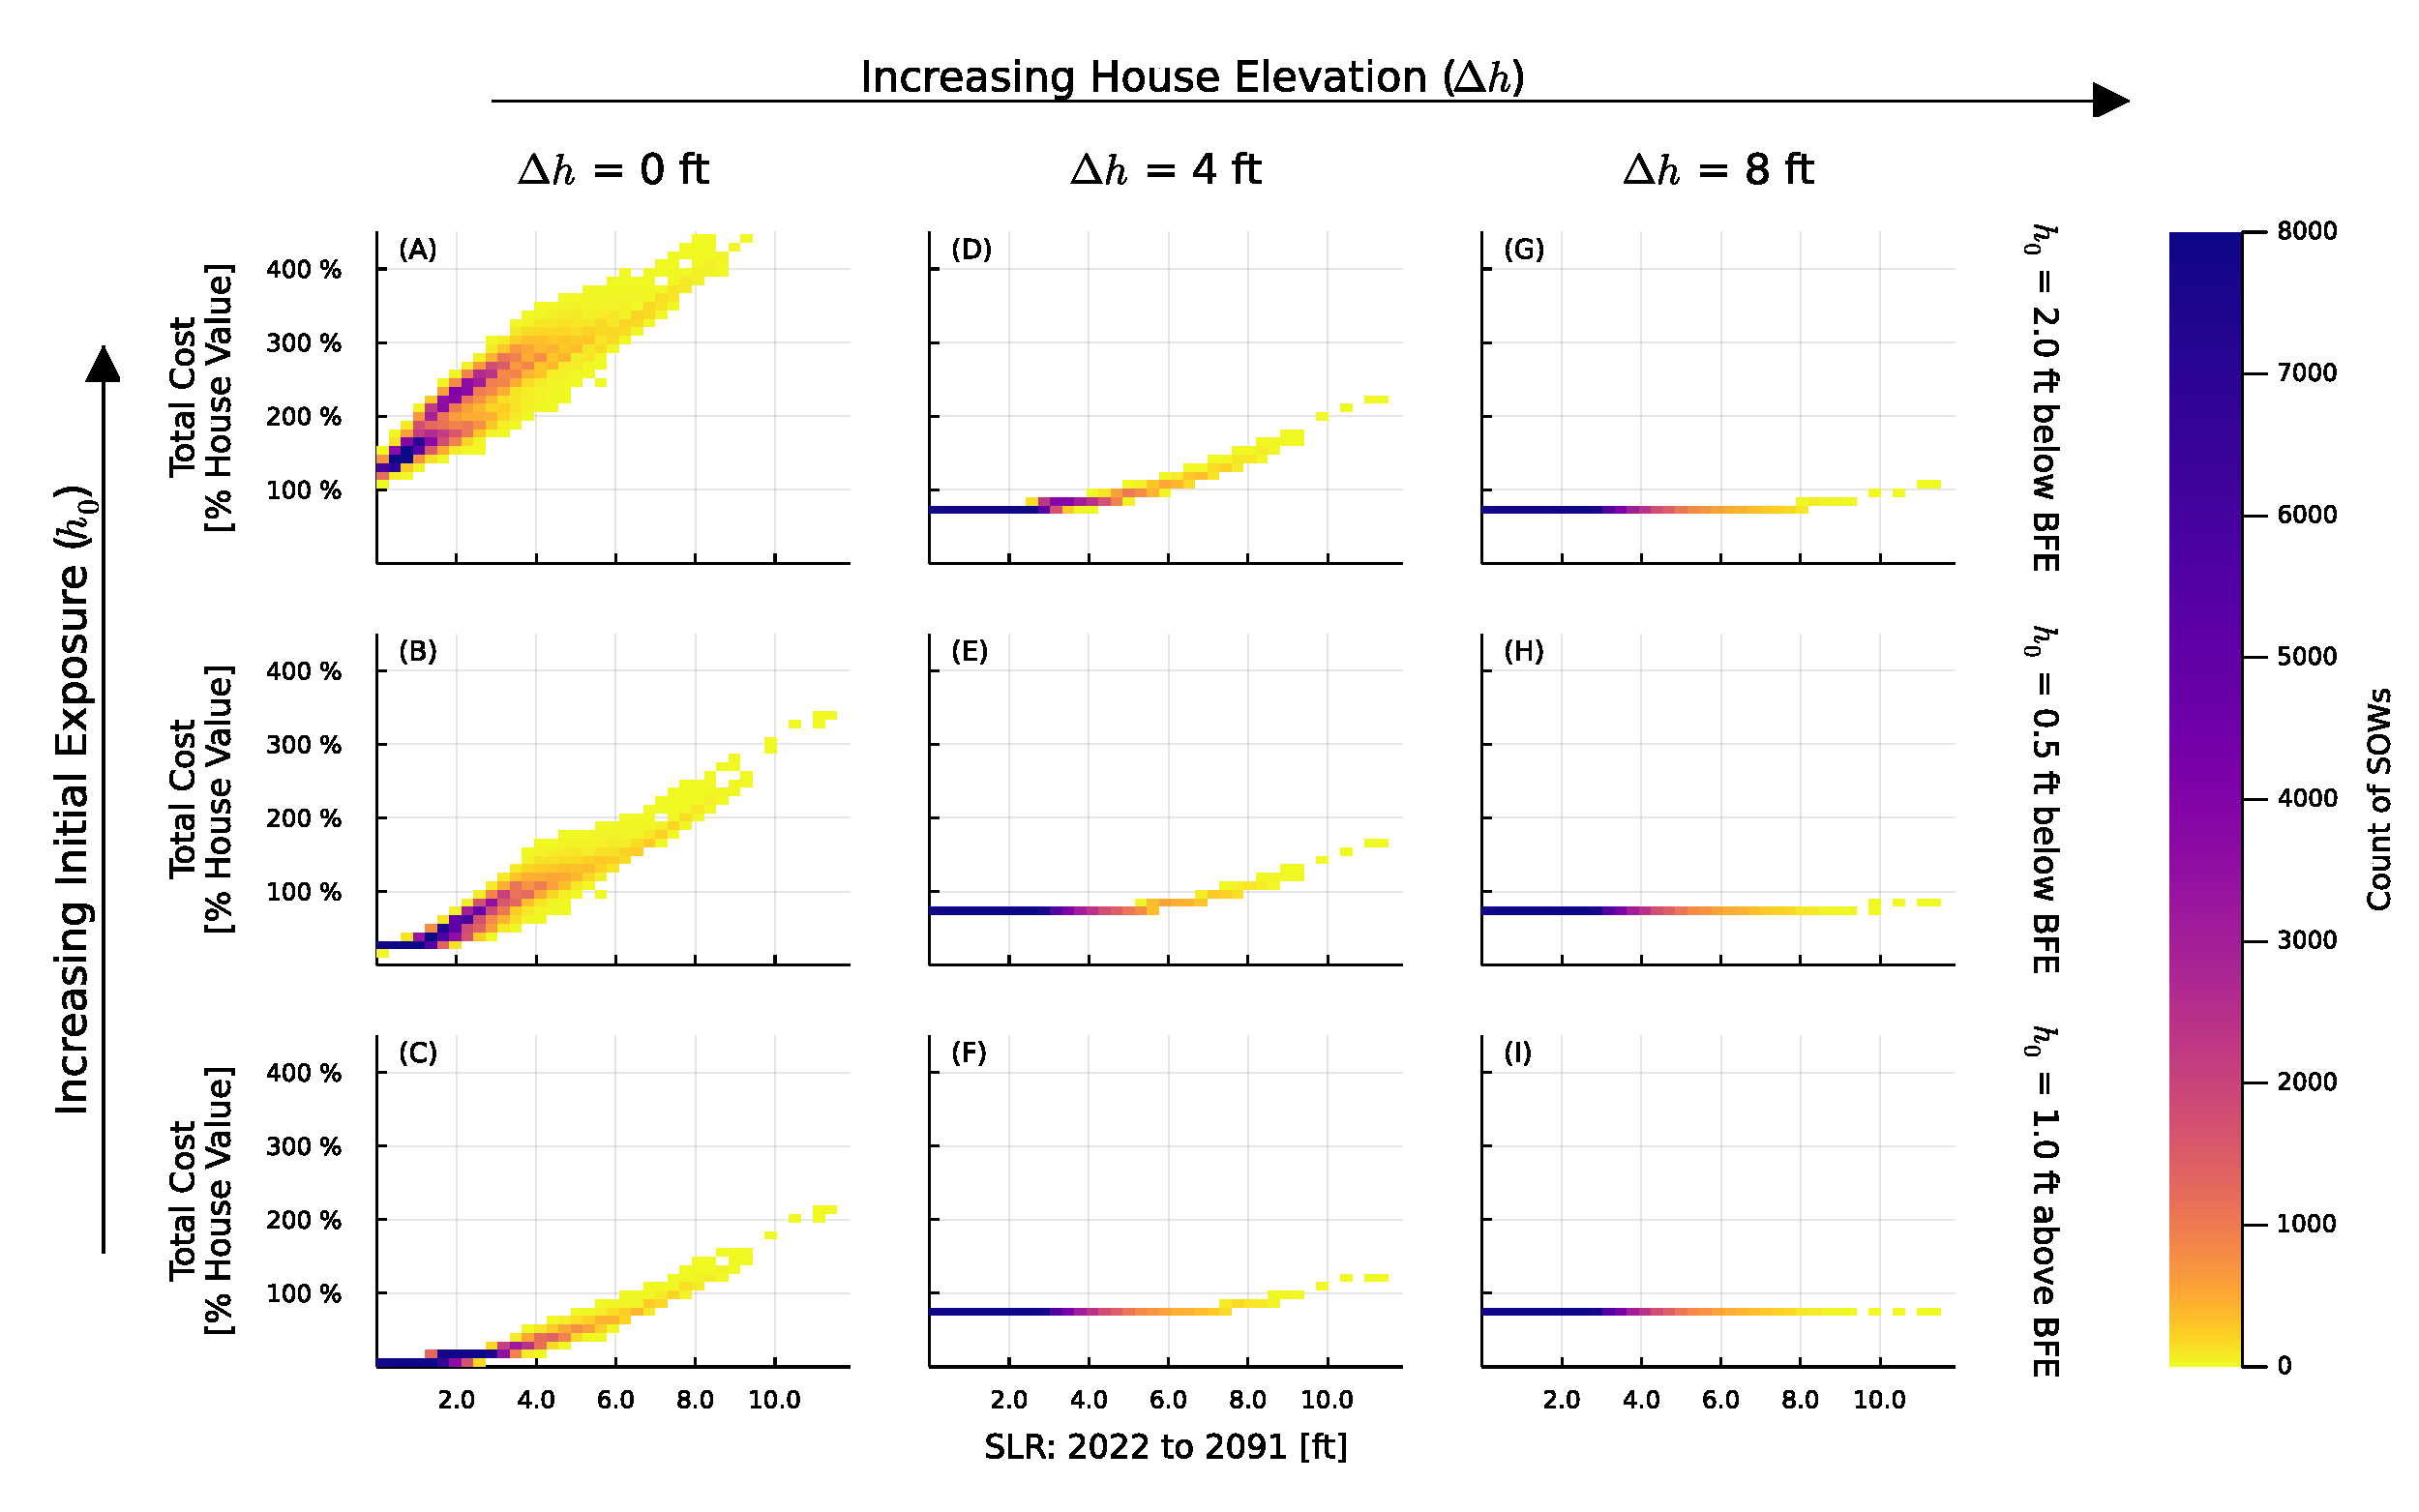
\includegraphics[width=\textwidth]{scenario-map-slr-cost}
  \caption{
    Scenario maps show the dependence of expected lifetime cost (damages plus up-front cost) as a function of \acrfull{msl} in 2100 for several values of initial height ($h_0$) and house elevation ($\Delta h$).
    Colors indicate the number of \acrfullpl{sow} of falling within each box.
    The lowest-cost outcomes occur when exposure is low ($h_0$ is large and \acrfull{slr} is minimal) and the house is not elevated (no up-front cost).
    The highest-cost outcomes arise when exposure is high ($h_0$ is small and \gls{slr} is rapid) and investment is inadequate.
    In all cases, elevating the house reduces the variance in total lifetime cost.
    Values are sensitive to model constants; see \cref{tab:uncertainties}.
  }\label{fig:scenario-map-slr-cost}
\end{figure}

One application of exploratory analysis is to reveal the range and variation in outcomes, conditional on taking a particular decision.
\Cref{fig:scenario-map-slr-cost} shows the dependence of expected lifetime costs (damages plus up-front costs; $y$-axis) as a function of  \gls{slr} over the house lifetime ($x$-axis), height increase ($\Delta h$; columns), and initial elevation ($h_0$; rows).
The outcomes with lowest total lifetime costs arise when the house is not elevated ($\Delta h = 0$) and \gls{slr} is minimal (bottom left corners).
The outcomes with highest total lifetime costs arise when the house is elevated only slightly and \gls{slr} is rapid.
As $\Delta h$ increases, the best-case scenario becomes more expensive because up-front costs increase, but worst-case scenarios become less expensive because even if \gls{slr} is substantial, damages will be negligible.

This analysis answers ``what-if'' questions like ``given $h_0$ and $\Delta h$, what is the range of total costs a homeowner could face if \gls{slr} over the house lifetime is \SI{1}{ft} or \SI{10}{ft}.''
For some decision-makers, contextualizing this information against a few scenarios of \gls{slr} \cite<\eg, those of>[]{sweet_slr:2022} may prove sufficient for decision making.
However, this analysis \DIFdelbegin \DIFdel{does not shed light on }\DIFdelend \DIFaddbegin \DIFadd{is silent on how to estimate }\DIFaddend cost-benefit \DIFdelbegin \DIFdel{analyses or }\DIFdelend \DIFaddbegin \DIFadd{comparisons, }\DIFaddend return periods, \DIFdelbegin \DIFdel{nor does it permit quantitative comparison against other possible decisions unless strong implicit assumptions are made}\DIFdelend \DIFaddbegin \DIFadd{and other trade-offs}\DIFaddend .

\subsection{Scenario-conditional \DIFdelbegin \DIFdel{optimization}\DIFdelend \DIFaddbegin \DIFadd{probabilistic analysis}\DIFaddend }\label{sec:results-conditional}

We now turn to the scenario-conditional analysis described in \cref{sec:analysis-condition}.
Whereas the exploratory analysis of the previous subsection interpreted each time series of future sea level as a sample from the space of possible futures, we can also interpret each \gls{sow} as a draw from one of the sixteen \DIFdelbegin \DIFdel{models }\DIFdelend \DIFaddbegin \DIFadd{probabilistic scenarios }\DIFaddend of \gls{slr} shown in \cref{fig:lsl-evolution}.
As discussed in \cref{sec:analysis-condition}, this allows a formal estimation of decision metrics, conditional on the chosen scenario.

\begin{figure}
  \centering
  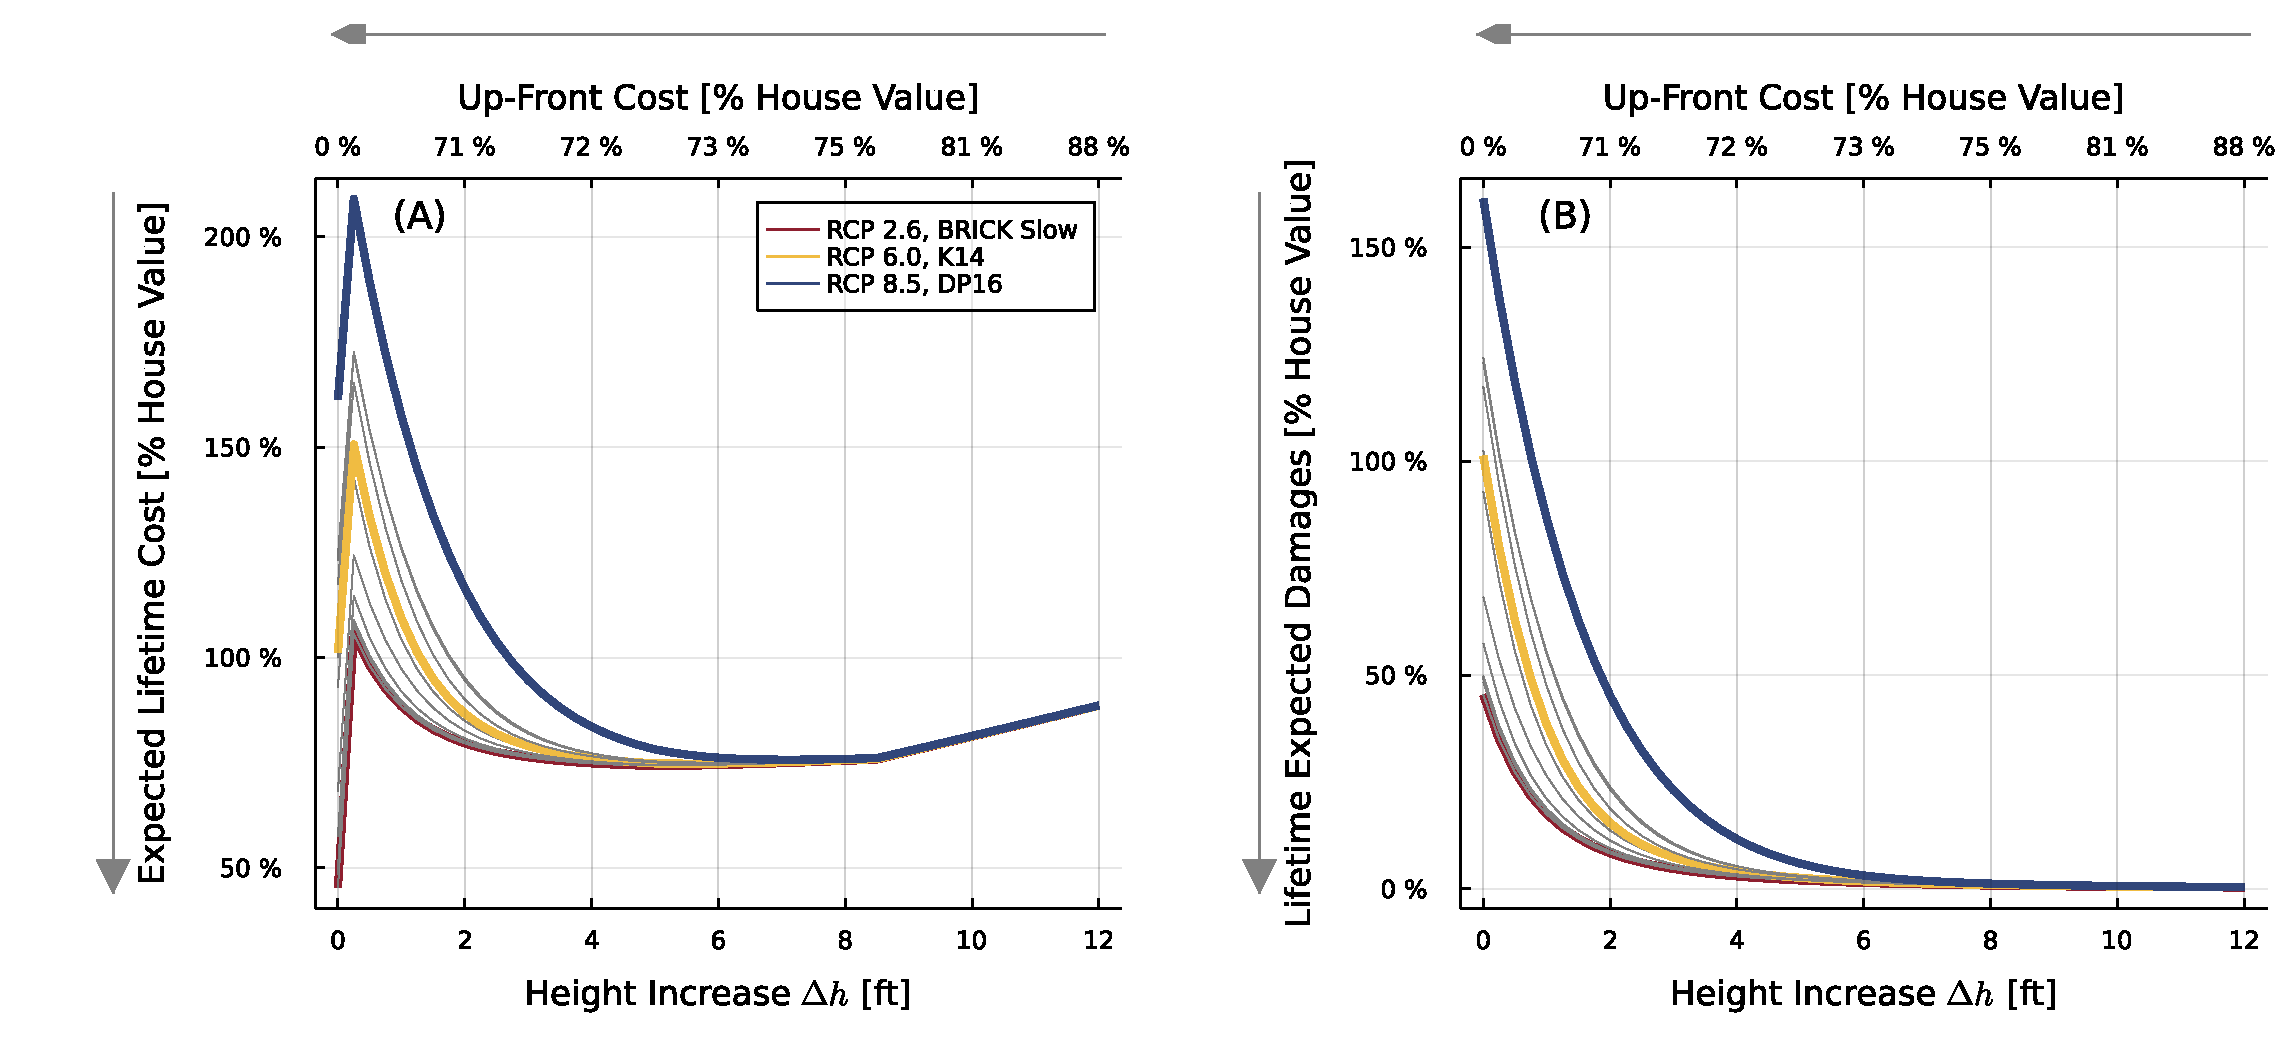
\includegraphics[width=\textwidth]{tradeoffs-by-rcp}
  \caption{
    Each probabilistic model or scenario leads to a different estimate of the Pareto frontier.
    For emphasis, we highlight three representative models: the Brick Slow model \protect\cite{wong_brick0.2:2017} under \gls{rcp} 2.6, the K14 \protect\cite{kopp_probabilistic:2014} model under \gls{rcp} 6.0 and the DP16 model \protect\cite{deconto_antarctica:2016,kopp_evolving:2017} under \gls{rcp} 8.5.
    (A): trade-off between up-front cost (which is a monotonic function of height increase) and expected lifetime costs.
    (B): trade-off between up-front cost and lifetime expected damages (eq.~\ref{eq:led}).
    Light gray lines show estimates for all 16 models (four \gls{rcp} scenarios times four physical parameterizations) considered.
    Colored lines highlight three representative models for emphasis.
    The gray arrows indicate the direction of preference.
  }\label{fig:tradeoffs-by-rcp}
\end{figure}


\DIFdelbegin \DIFdel{This }\DIFdelend \DIFaddbegin \DIFadd{As discussed in \mbox{%DIFAUXCMD
    \cref{sec:analysis-condition}}\hskip0pt%DIFAUXCMD
  , this }\DIFaddend probabilistic interpretation allows us to compute \DIFdelbegin \DIFdel{, for example, expected values }\DIFdelend \DIFaddbegin \DIFadd{expected values of functions}\DIFaddend .
For example, \cref{fig:tradeoffs-by-rcp}(a) plots the expected total lifetime cost as a function of $\Delta h$ for the sixteen \DIFdelbegin \DIFdel{models }\DIFdelend \DIFaddbegin \DIFadd{probabilistic scenarios }\DIFaddend considered (we highlight three representative models).
\DIFdelbegin \DIFdel{Similarly, \mbox{%DIFAUXCMD
    \cref{fig:tradeoffs-by-rcp}}\hskip0pt%DIFAUXCMD
  (b) plots the }\DIFdelend \DIFaddbegin \DIFadd{This panel shows }\DIFaddend lifetime expected damages as a function of $\Delta h$\DIFdelbegin \DIFdel{.
}\DIFdelend \DIFaddbegin \DIFadd{, shown in \mbox{%DIFAUXCMD
    \cref{fig:tradeoffs-by-rcp}}\hskip0pt%DIFAUXCMD
  (b,  plus the up-front cost of construction.
  Because there are high fixed costs associated with building (see cost curve in fig.~S3), it generally does not make sense to raise the house by only a small amount, since this incurs these fixed costs without providing substantial damage reduction.
  \mbox{%DIFAUXCMD
    \Cref{fig:tradeoffs-by-rcp} }\hskip0pt%DIFAUXCMD
  shows that estimates of trade-offs between up-front cost and expected lifetime costs are highly sensitive to the chosen scenario.
}\DIFaddend For small $\Delta h$, expected costs are low under optimistic \DIFdelbegin \DIFdel{models }\DIFdelend \DIFaddbegin \DIFadd{scenarios }\DIFaddend (\eg, \gls{rcp} 2.6 with slow ice sheet dynamics; red lines) and high under pessimistic \DIFdelbegin \DIFdel{models }\DIFdelend \DIFaddbegin \DIFadd{scenarios }\DIFaddend (\eg, \gls{rcp}8.5 with the DP16 model; blue lines).
\DIFaddbegin \DIFadd{Estimates of the optimal decision are highly sensitive to the choice of scenario.
}\DIFaddend For example, under the most pessimistic \DIFdelbegin \DIFdel{model }\DIFdelend \DIFaddbegin \DIFadd{scenario }\DIFaddend (blue line), the cost-minimizing height increase is \SI{6}{ft}, which incurs an up-front cost of 73\% of the house value but reduces lifetime expected damages by over 150\% of house value.
Under the most optimistic \DIFdelbegin \DIFdel{model }\DIFdelend \DIFaddbegin \DIFadd{scenario }\DIFaddend (gray line), the cost-minimizing decision is to not elevate, as elevating \SI{6}{ft} incurs the same up-front cost yet reduces lifetime expected damages by less than 50\% of house value.

This approach is, in a sense, another form of exploratory modeling: instead of considering a very large ensemble of \glspl{sow}, we consider a much smaller set of probabilistic models.
\DIFdelbegin \DIFdel{This approach is }\DIFdelend \DIFaddbegin \DIFadd{Scenario-conditional analysis can be }\DIFaddend attractive because it allows modelers to focus on their domain expertise (\eg, the response of ice sheets and global sea levels to a particular climate future).
However, conditioning simulations on a set of climate futures and physical models presents what we term ``the multiple \gls{pdf} problem'' because it leaves decision makers with many \glspl{pdf} to choose from and hence many trade-off curves to navigate.
The multiple \gls{pdf} problem has also been \DIFdelbegin \DIFdel{shown }\DIFdelend \DIFaddbegin \DIFadd{discussed }\DIFaddend in other contexts.
For example, \citeA{sharma_rcp:2021} model the reliability of stormwater infrastructure under different climate models and downscaling methods, finding diverging estimates of future rainfall hazard, even under a single \gls{rcp} scenario.
Similarly, \citeA{wong_nola:2017} construct 18 probability distribution functions for future flood risk in New Orleans, considering multiple models for ice sheet dynamics and storm surge and multiple \gls{rcp} scenarios. As a last example, \citeA{haasnoot_sealevelrise:2021} identify global adaptation needs for different \gls{slr} scenarios.
Although this scenario-conditional analysis is appropriate for understanding differences between models, its key limitation is that it \textbf{places the burden for deciding which model to design for onto the end user.}
\DIFaddbegin \DIFadd{Since not all house owners or contractors have expertise in assessing the relative likelihood of different climate futures, they may not be well positioned to make this decision.
}\DIFaddend

\subsection{Synthesizing deep uncertainties for decision analysis}\label{sec:results-synthesis}

The \DIFdelbegin \DIFdel{proposed approach }\DIFdelend \DIFaddbegin \DIFadd{\mbox{%DIFAUXCMD
    \gls{sow} }\hskip0pt%DIFAUXCMD
  re-weighting framework described in \mbox{%DIFAUXCMD
    \cref{sec:reweighting} }\hskip0pt%DIFAUXCMD
}\DIFaddend can help overcome the limitations of scenario-conditional analysis.
\DIFdelbegin \DIFdel{We illustrate how the re-weighting method described in \mbox{%DIFAUXCMD
    \cref{sec:analysis-synthesize} }\hskip0pt%DIFAUXCMD
}\DIFdelend \DIFaddbegin \DIFadd{In this section we illustrate how this approach }\DIFaddend can help to shed light on climate risk management under deep uncertainty.
We present results using each of the models for $p_\mathrm{belief}$ outlined in \cref{sec:case-priors}\DIFdelbegin \DIFdel{.
  These }\DIFdelend \DIFaddbegin \DIFadd{; these }\DIFaddend three distributions are shown in \cref{fig:lsl-priors-weights}(A).

\begin{figure}
  \centering
  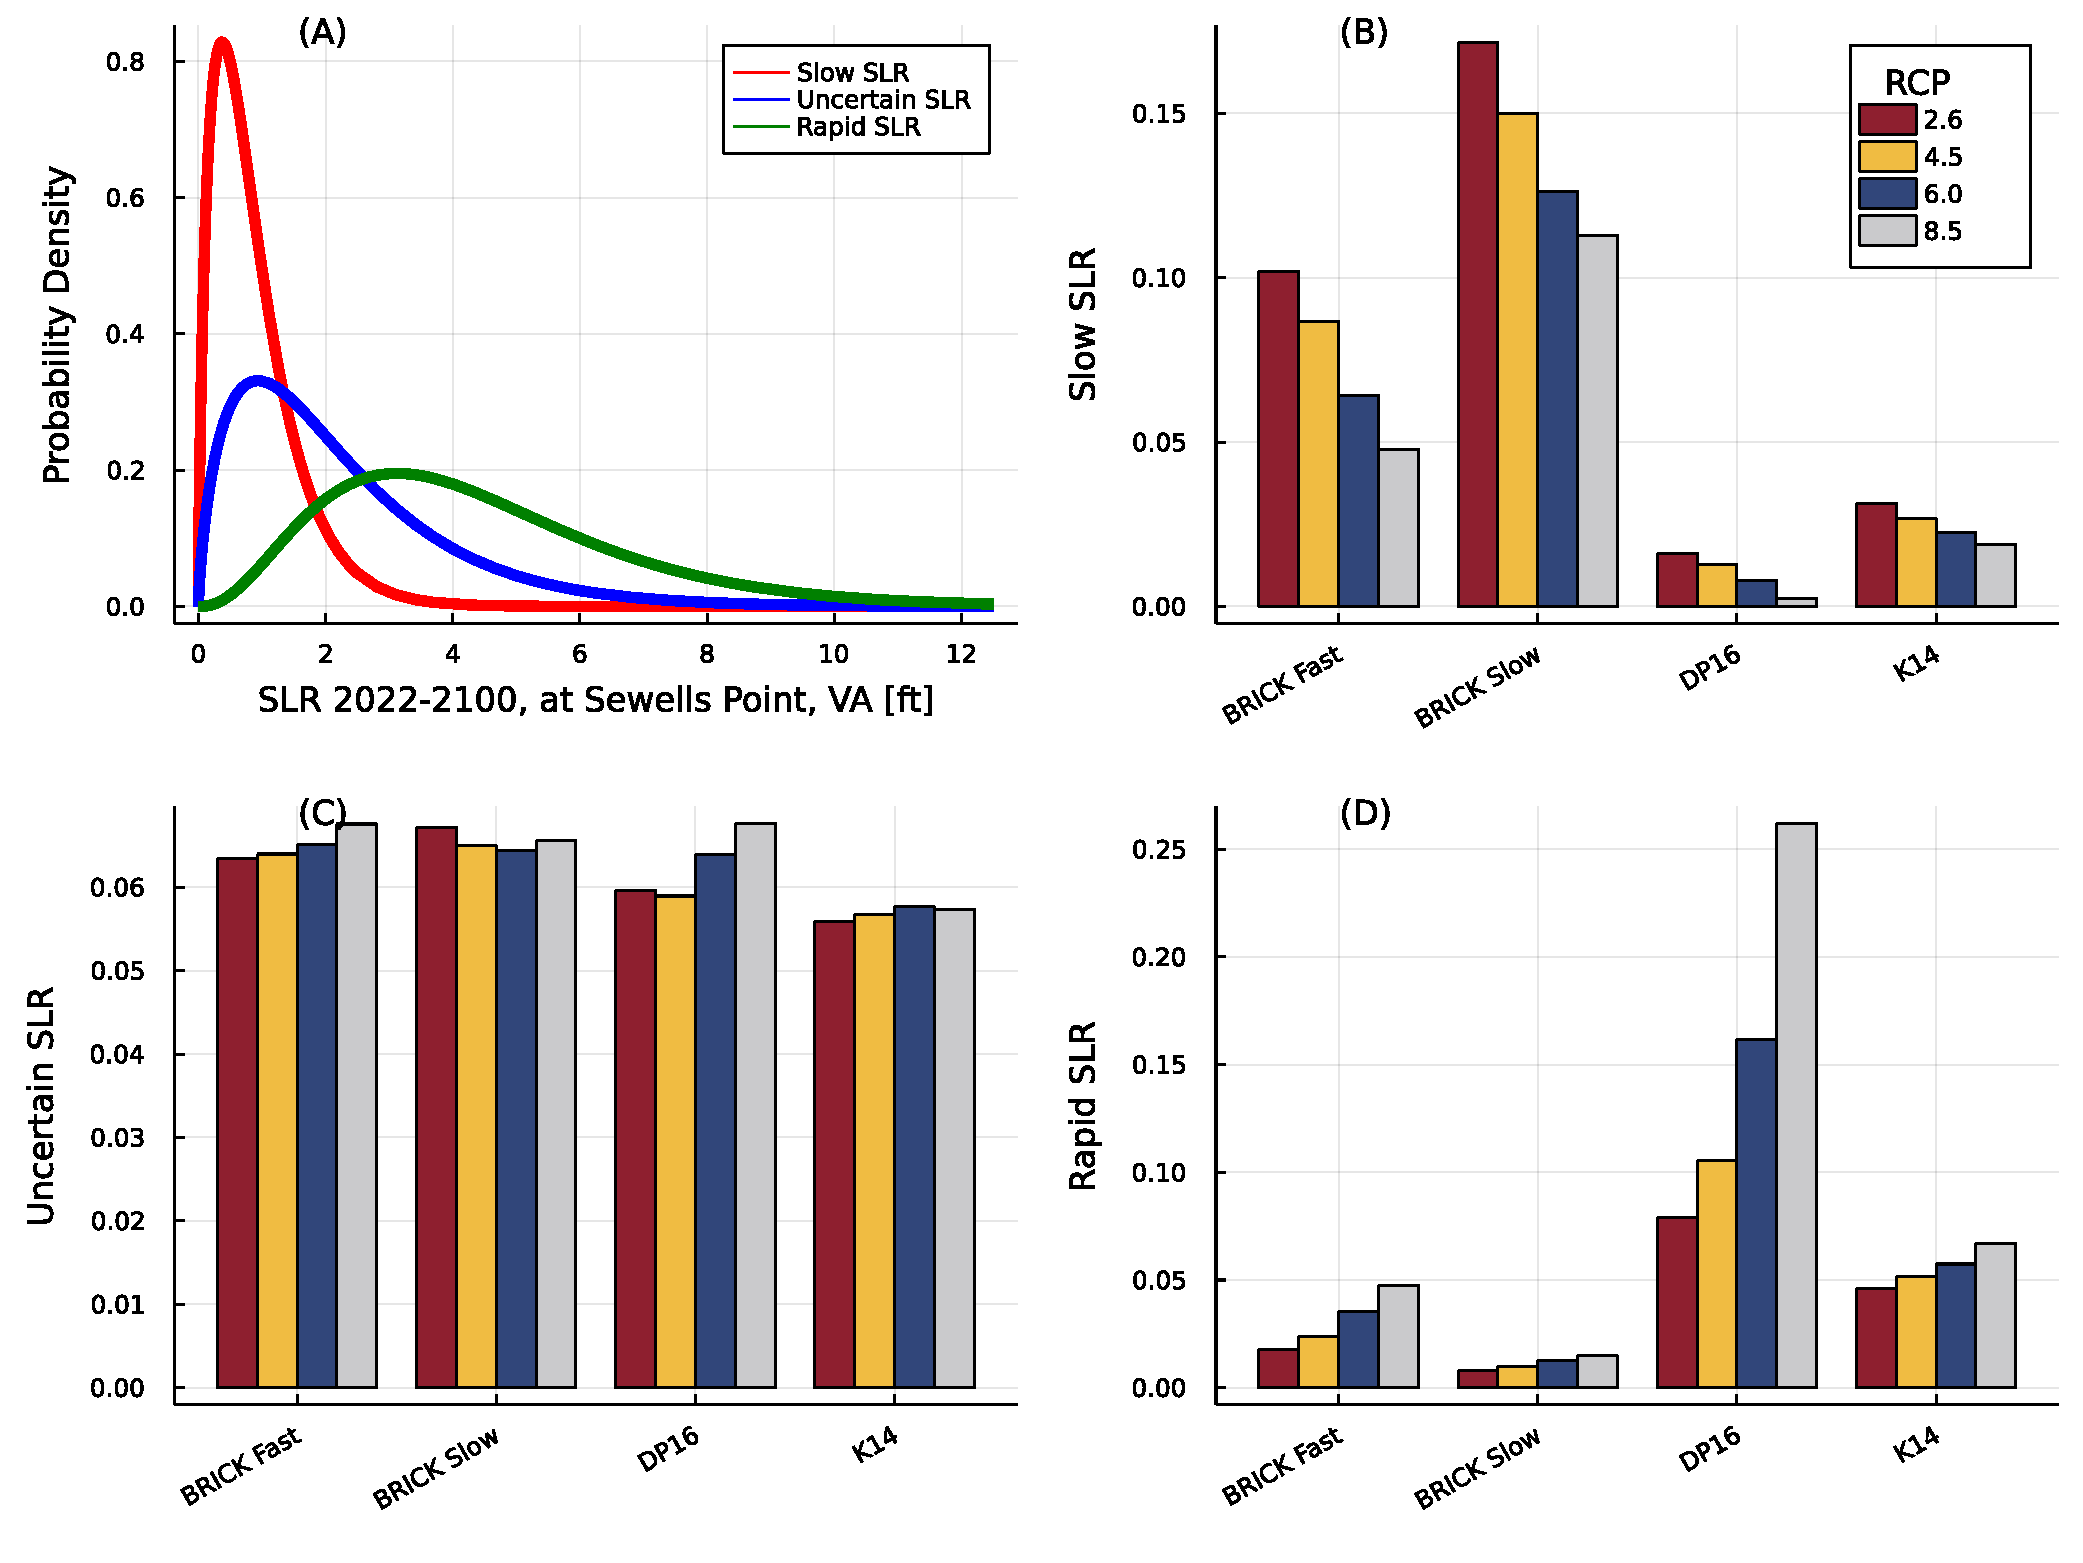
\includegraphics[width=\textwidth]{lsl-priors-weights}
  \caption{
    Impact of \DIFaddbeginFL \DIFaddFL{different }\DIFaddendFL subjective \DIFdelbeginFL \DIFdelFL{priors }\DIFdelendFL \DIFaddbeginFL \DIFaddFL{probability distributions }\DIFaddendFL for local sea level on implicit weight given to each \gls{rcp} scenario and physical model.
    We develop three distributions \DIFdelbeginFL \DIFdelFL{(``subjective priors'') }\DIFdelendFL representing plausible probabilistic beliefs \DIFdelbeginFL \DIFdelFL{about }\DIFdelendFL \DIFaddbeginFL \DIFaddFL{($p_\mathrm{belief}$) over }\DIFaddendFL \gls{msl} at Sewells Point, VA in 2100, relative to the present.
    The \glspl{pdf} of these \DIFdelbeginFL \DIFdelFL{subjective priors }\DIFdelendFL \DIFaddbeginFL \DIFaddFL{distributions }\DIFaddendFL are shown in panel (A).
    In panels (B-C) we show the relationship between these \DIFdelbeginFL \DIFdelFL{subjective priors }\DIFdelendFL \DIFaddbeginFL \DIFaddFL{distributions }\DIFaddendFL and the 16 probabilistic models (four \gls{rcp} scenarios and four physical representations) available.
    Specifically, (B-C) show the average weight given to each model by each \DIFdelbeginFL \DIFdelFL{of the subjective priors}\DIFdelendFL \DIFaddbeginFL \DIFaddFL{choice for $p_\mathrm{belief}$}\DIFaddendFL .
  }\label{fig:lsl-priors-weights}
\end{figure}

One application of this method is to diagnose \DIFdelbegin \DIFdel{which assumptions }\DIFdelend \DIFaddbegin \DIFadd{the assumptions which which }\DIFaddend different $p_\mathrm{belief}$ are consistent\DIFdelbegin \DIFdel{with}\DIFdelend .
\Cref{fig:lsl-priors-weights}(B-D) shows the total weight that each \DIFdelbegin \DIFdel{prior }\DIFdelend \DIFaddbegin \DIFadd{choice of $p_\mathrm{belief}$ }\DIFaddend assigns to \glspl{sow} generated by each \gls{rcp} scenario and physical model.
\DIFaddbegin \DIFadd{Specifically, weights are computed as the sum of weights assigned to each \mbox{%DIFAUXCMD
    \gls{sow} }\hskip0pt%DIFAUXCMD
  sampled from that model.
}\DIFaddend For example, the rapid \gls{slr} scenario (green line in \cref{fig:lsl-priors-weights}) places most weight on \DIFaddbegin \DIFadd{\mbox{%DIFAUXCMD
    \glspl{sow} }\hskip0pt%DIFAUXCMD
  produced by }\DIFaddend the DP16 model, and particularly on \gls{rcp} 8.5 which by some accounts is unlikely given current policy \cite{hausfather_scenarios:2020,srikrishnan_probabilistic:2022}.
Conversely, the slow \gls{slr} scenario (red line) places most weight on the BRICK models, particularly \gls{rcp} 2.6 \cite<also unlikely given current policy;>{hausfather_scenarios:2020,srikrishnan_probabilistic:2022} \DIFdelbegin \DIFdel{) }\DIFdelend and \gls{rcp} 4.5.
The uncertain \gls{slr} scenario (blue line) allocates approximately equal weight across models.
\DIFaddbegin \DIFadd{Decision analysts can use this approach as a diagnostic to understand the assumptions implicit to their choice of $p_\mathrm{belief}$.
}\DIFaddend

This method can also be used to calculate expectations, allowing us to revisit the trade-off diagrams of \cref{fig:tradeoffs-by-rcp}.
\Cref{fig:tradeoffs-by-prior} shows the total lifetime cost (panel A) and lifetime expected damages (panel B) under each \DIFdelbegin \DIFdel{model}\DIFdelend \DIFaddbegin \DIFadd{choice of $p_\mathrm{belief}$}\DIFaddend .
Notably, they give different guidance.
Under an assumption of rapid \gls{slr}, elevating the house by approximately \SI{6}{ft} costs 73\% of house value and reduces damages by over 100\% of house value, yielding a benefit to cost ratio of approximately 1.25.
Under an assumption of slow \gls{slr}, the same decision reduces damages only by 50\% of house value, yielding a benefit to cost ratio of approximately 0.7.
Under the intermediate / uncertain \gls{slr} assumption, the expected lifetime costs are similar for elevating or not elevating the house, and thus the benefit to cost ratio is nearly 1.
Under all assumptions, elevating by only a few feet is impractical because it involves paying the large fixed costs of elevation (\DIFdelbegin \DIFdel{\mbox{%DIFAUXCMD
    \cref{fig:cost-up-front}}\hskip0pt%DIFAUXCMD
}\DIFdelend \DIFaddbegin \DIFadd{fig.~S3}\DIFaddend ) but offers relatively little flood reduction.
\DIFaddbegin \DIFadd{Based on this analysis, we would recommend that the owner if this hypothetical home elevate by approximately 4-6}\si{ft} \DIFadd{or not at all.
  Alternatively, the homeowner could choose to defer the decision of whether, and how high, to elevate; our analysis did not consider this possibility but there is a rich literature on flexible design and engineering options analysis in climate risk analysis \mbox{%DIFAUXCMD
    \cite<\eg,>{fletcher_learning:2019,fletcher_groundwater:2019,hui_adaptive:2018,garner_slrise:2018,herman_control:2020,deneufville_eoa_theory:2019}}\hskip0pt%DIFAUXCMD
  .
}\DIFaddend

\begin{figure}
  \centering
  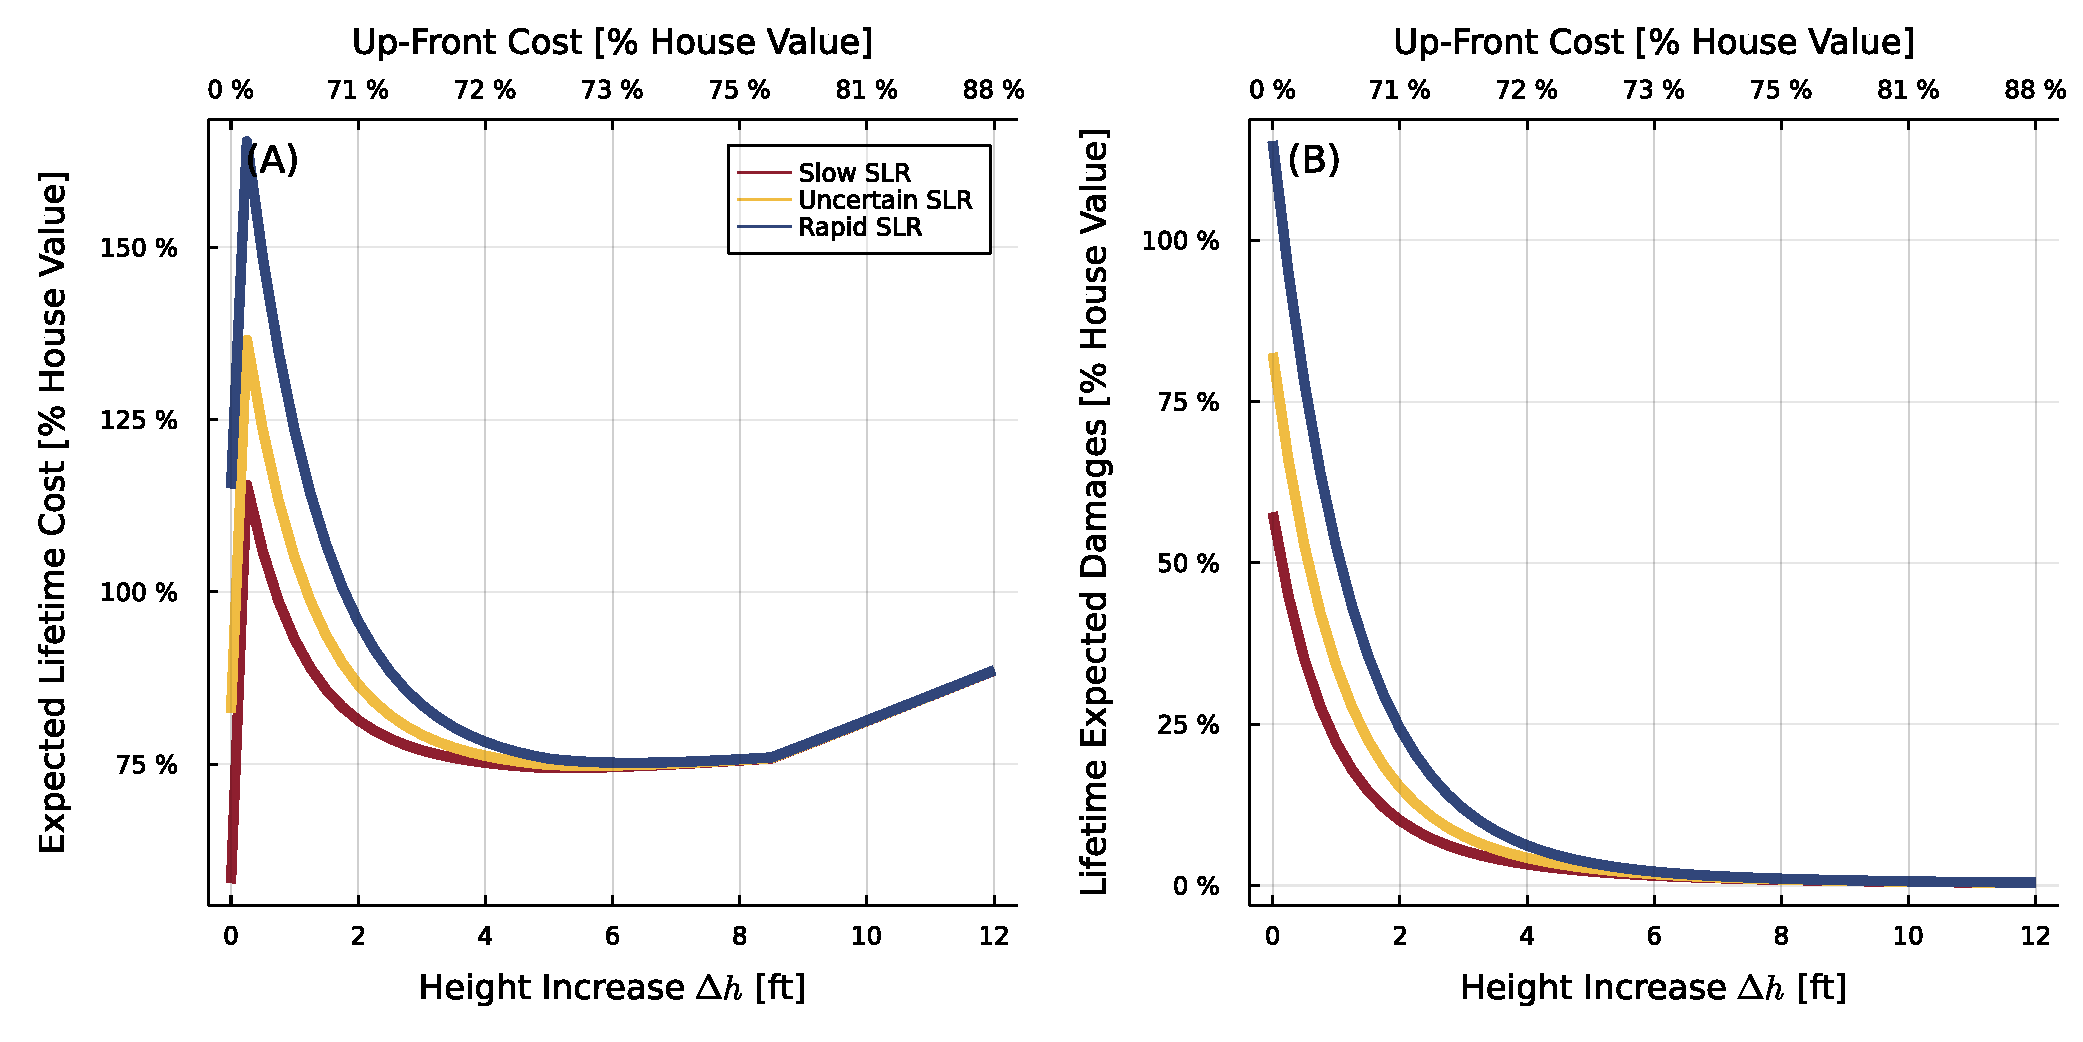
\includegraphics[width=\textwidth]{tradeoffs-by-prior}
  \caption{
    As \cref{fig:tradeoffs-by-rcp}, but with Pareto frontiers for the full distribution of outcomes using the three models of $p_\mathrm{belief}$ (colors).
  }\label{fig:tradeoffs-by-prior}
\end{figure}

\section{\DIFdelbegin \DIFdel{Discussion }\DIFdelend \DIFaddbegin \DIFadd{Limitations }\DIFaddend and research needs}\label{sec:caveats}

Several limitations to our study merit further discussion.
The first category has to do with limitations of the underlying method proposed for re-weighting \glspl{sow}.
For example, we develop a subjective \DIFdelbegin \DIFdel{prior belief }\DIFdelend \DIFaddbegin \DIFadd{probabilistic model }\DIFaddend $p_\mathrm{belief}(\Psi)$ over \gls{msl} in the year 2100.
Although this is a low-dimensional representation of the full time series, it is not a sufficient statistic\DIFdelbegin \DIFdel{; prior studies have shown that using Approximate Bayesian Computation to calibrate models on low dimensional statistics using that are not sufficient statistics can lead to biased posterior estimates \mbox{%DIFAUXCMD
    \cite{csillery_abc:2010,marjoram_abc:2006}}\hskip0pt%DIFAUXCMD
  .
  Although we are not performing calibration here,  and this is thus not a direct concern, }\DIFdelend \DIFaddbegin \DIFadd{.
  In other words,  many possible low-dimensional representations are possible and }\DIFaddend time series with the same \gls{msl} in 2100 may differ in other ways\DIFdelbegin \DIFdel{, and experts may have prior information about the likelihood of these differences not represented in our model}\DIFdelend \DIFaddbegin \DIFadd{.
  For problems with more sources of uncertainty, such as multisector problems, choosing an appropriate low-dimensional representation may prove challenging.
  In such settings, diagnostics and sensitivity analyses may shed light on the appropriateness of different modeling choices}\DIFaddend .
A related concern is that we developed our three distributions for $p_\mathrm{belief}(\Psi)$  in an \emph{ad hoc} fashion that may not represent well-calibrated beliefs.
Although this is appropriate for our didactic illustration, recent advances in Bayesian elicitation of expert opinion \cite<see>[and references therein]{mikkola_elicitation:2021} can be applied to improve decision making in real world case studies.
More fundamentally, our method assumes that there exists an expert capable of integrating over the many processes that drive \gls{slr}, from global greenhouse gas emissions to the global carbon cycle to climate sensitivity and ice sheet response \cite{morgan_elicitation:2014}.
An alternative approach would be to build a probabilistic model for each of these steps, and to use each as an input to the next to develop a fully probabilistic model for \gls{slr}.
Yet while some progress has been made developing probabilistic models for specific elements of this model chain \cite<\eg,>[]{srikrishnan_probabilistic:2022,wong_brick0.2:2017}, this remains a computational and conceptual challenge.
\DIFdelbegin \DIFdel{Finally, while our aim in this paper has been to demonstrate the value of integrating Bayesian workflow \mbox{%DIFAUXCMD
    \cite{gelman_workflow:2020} }\hskip0pt%DIFAUXCMD
  into \mbox{%DIFAUXCMD
    \gls{dmdu}}\hskip0pt%DIFAUXCMD
  , further work is needed to improve this integration.
}\DIFdelend

The second category of limitations has to do with the case study and our interpretation of the house elevation decision problem.
This problem intersects with decisions about where to live and how to manage household finances, both of which are highly complex.
One extension of our analysis would be to consider additional decision objectives.
In particular, we hypothesize that incorporating improved representations of risk aversion into decision support may substantially improve their usability.
One could also extend the analysis to consider additional sources of uncertainty such as depth-damage relationships \cite{Rozer:2019,nofal_fragility:2020}, the cost of elevating a house, the house lifespan, the effective discount rate, and value of the land on which the house is built \DIFdelbegin \DIFdel{\mbox{%DIFAUXCMD
    \cite[provides a framework for addressing some of these]{zarekarizi_suboptimal:2020}}\hskip0pt%DIFAUXCMD
}\DIFdelend \DIFaddbegin \DIFadd{\mbox{%DIFAUXCMD
    \cite{zarekarizi_suboptimal:2020}}\hskip0pt%DIFAUXCMD
}\DIFaddend .
Finally, while here we consider the decision to be a one-time decision, one could also frame this as \DIFdelbegin \DIFdel{problem }\DIFdelend a sequential decision \DIFaddbegin \DIFadd{problem}\DIFaddend .
The analysis of sequential decision problems applies tools from control theory and reinforcement learning to identify policies that map ``triggers'' (\ie, state variables) to decisions \cite{herman_control:2020}.
Yet although framing the decision through a sequential lens can increase adaptability and improve outcomes \cite{fletcher:2017,garner_slrise:2018}, \DIFdelbegin \DIFdel{the optimized policy rules are necessarily }\DIFdelend \DIFaddbegin \DIFadd{decisions and outcomes remain highly }\DIFaddend sensitive to the characterization of uncertainty \DIFaddbegin \DIFadd{\mbox{%DIFAUXCMD
    \cite{herman_control:2020}}\hskip0pt%DIFAUXCMD
}\DIFaddend , and thus the problem of synthesizing across deep uncertainties remains \DIFdelbegin \DIFdel{\mbox{%DIFAUXCMD
    \cite{herman_control:2020}}\hskip0pt%DIFAUXCMD
}\DIFdelend \DIFaddbegin \DIFadd{relevant}\DIFaddend .

These limitations motivate several directions for future research.
From a methodological perspective, developing model chains that capture uncertainties in global energy and economic pathways, global climate sensitivity, and local hazard response \cite<see fig.~1 of>[]{moss_uncertainties:2000} offers a principled framework for fully probabilistic estimation of local hazard, subject to (still necessarily subjective) \DIFdelbegin \DIFdel{priors over }\DIFdelend \DIFaddbegin \DIFadd{probabilistic models for }\DIFaddend key parameters.
From a decision support perspective, improved understanding of the conditions under which household-scale strategies for flood risk management, like elevation, achieve relevant objectives could support improved resilience and adaptation.
Additionally, since developing bespoke analyses for each house may be impractical, identifying decision rules that are applicable across different house characteristics may improve usability \DIFdelbegin \DIFdel{.
}\DIFdelend \DIFaddbegin \DIFadd{and guidance.
  Finally, there are many parallels between \mbox{%DIFAUXCMD
    \gls{dmdu} }\hskip0pt%DIFAUXCMD
  and subjective Bayesian literature on building predictive models in the ``$\mathcal{M}$-closed'' case when ``all models are wrong'' \mbox{%DIFAUXCMD
    \cite{gelman_philosophy:2013,box_sciencestatistics:1976}}\hskip0pt%DIFAUXCMD
  , and thus future work can demonstrate how to incorporate techniques from Bayesian workflow \mbox{%DIFAUXCMD
    \cite<see>{gelman_workflow:2020} }\hskip0pt%DIFAUXCMD
  into \mbox{%DIFAUXCMD
    \gls{dmdu} }\hskip0pt%DIFAUXCMD
  methodologies.
}\DIFaddend

\section{Conclusions}\label{sec:conclusions}

This study develops a framework designed to increase the transparency of quantitative decision analysis under deep uncertainty.
We develop a framework capable of blending iterative, stakeholder-driven exploratory modeling \DIFaddbegin \DIFadd{\mbox{%DIFAUXCMD
    \cite<see, \eg,>{helgeson_manifesto:2022} }\hskip0pt%DIFAUXCMD
}\DIFaddend with subjective probabilistic expert assessment.
Such an approach is urgently needed given that deeply uncertain nonstationarity hazards pose a fundamental challenge to classical methods of hazard estimation.
We use a didactic case study of house elevation in the coastal zone to illustrate a method for transparently synthesizing across deep uncertainties.

The proposed \DIFdelbegin \DIFdel{scenario weighting }\DIFdelend \DIFaddbegin \DIFadd{\mbox{%DIFAUXCMD
    \gls{sow} }\hskip0pt%DIFAUXCMD
  re-weighting }\DIFaddend framework can be applied to inform critical challenges in climate risk management.
An obvious area of application is to the design of infrastructure.
For example, much of the stormwater infrastructure in the United States is inadequate for current and anticipated future climates \cite{lopez-cantu:2018}.
Yet upgrading this infrastructure is costly and subject to large uncertainties between rainfall models \cite{sharma_rcp:2021} and \gls{rcp} scenarios.
Similarly, decisions like  levee heightening \cite{garner_slrise:2018,oddo_coastal:2017,vandantzig_dike:1956} and sea wall design \DIFdelbegin \DIFdel{(as discussed in the Introduction) }\DIFdelend \DIFaddbegin \DIFadd{\mbox{%DIFAUXCMD
    \cite[Appendix D.,~p.~2-59]{USACE_coastal:2021} }\hskip0pt%DIFAUXCMD
}\DIFaddend are subject to deep uncertainties \DIFdelbegin \DIFdel{in }\DIFdelend \DIFaddbegin \DIFadd{including }\DIFaddend sea level rise.
Investments in water resources planning and management \DIFaddbegin \DIFadd{also }\DIFaddend depend on assumptions of future water demand, availability, and technologies \cite{trindade_deeplyuncertainpathways:2019}.
And analyses of climate change mitigation options, such as estimates of the social cost of pollutants \cite{errickson_methane:2021} or cost-minimizing energy transition pathways, are conditional on probabilistic models for inputs like technology prices and population.

Of course, all models are ultimately wrong \cite{box_sciencestatistics:1976}.
Thus seeking decisions that perform well across a range of assumptions, and improving the decision space through robust design and flexibility, can improve outcomes.
Yet whenever decisions are compared quantitatively, assumptions about the probability of different possible futures are necessarily made.
We call for researchers studying climate risk management to make these implicit assumptions explicit, and we suggest that coordinated guidance can help practitioners determine better design criteria.

\section{Open Research}

All code, including source code, is available under the GNU Public License (version 3) at \url{https://github.com/jdossgollin/2022-elevation-robustness}.
This code is written in the open source Julia programming language and detailed instructions for reproducing our results are provided.
A permanent, citeable archive of the precise version of the codes used in this study is also available on Zenodo at \url{https://doi.org/10.5281/zenodo.6814588}.

%%%%%%%%%%%%%%%%%%%%%%%%%%%%%%%%%%%%%%%%%%%%%%%

\acknowledgments

This work was supported by \acrfull{noaa} through the Mid-Atlantic Regional Integrated Sciences and Assessments (MARISA) program under \gls{noaa} grant NA16OAR4310179 and through the Penn State Initiative for Resilient Communities (PSIRC) by a Strategic Plan seed grant from the Penn State Office of the Provost, with co-support from the Center for Climate Risk Management (CLIMA), the Rock Ethics Institute, Penn State Law, and the Hamer Center for Community Design.
JDG thanks Rice University for support.
KK thanks Dartmouth College for support.
The authors thank
Sitara Baboolal,
\DIFaddbegin \DIFadd{Courtney Cooper,
}\DIFaddend Tor Erlend Fjelde,
Catalina González-Dueñas,
Adam Pollack,
\DIFdelbegin \DIFdel{and
  Vivek Srikrishnan}\DIFdelend \DIFaddbegin \DIFadd{Vivek Srikrishnan,
  Skip Wishbone,
  and two anonymous peer reviewers
}\DIFaddend for helpful comments \DIFaddbegin \DIFadd{that improved this research}\DIFaddend .


%% ------------------------------------------------------------------------ %%
%% References and Citations
% don't specify bibliographystyle
% In the References section, cite the data/software described in the Availability Statement (this includes primary and processed data used for your research). For details on data/software citation as well as examples, see the Data & Software Citation section of the Data & Software for Authors guidance
% https://www.agu.org/Publish-with-AGU/Publish/Author-Resources/Data-and-Software-for-Authors#citation

%%%%%%%%%%%%%%%%%%%%%%%%%%%%%%%%%%%%%%%%%%%%%%%

\bibliography{library-bibtex}


\end{document}
